% Options for packages loaded elsewhere
% Options for packages loaded elsewhere
\PassOptionsToPackage{unicode}{hyperref}
\PassOptionsToPackage{hyphens}{url}
\PassOptionsToPackage{dvipsnames,svgnames,x11names}{xcolor}
%
\documentclass[
  twocolumn]{article}
\usepackage{xcolor}
\usepackage{amsmath,amssymb}
\setcounter{secnumdepth}{5}
\usepackage{iftex}
\ifPDFTeX
  \usepackage[T1]{fontenc}
  \usepackage[utf8]{inputenc}
  \usepackage{textcomp} % provide euro and other symbols
\else % if luatex or xetex
  \usepackage{unicode-math} % this also loads fontspec
  \defaultfontfeatures{Scale=MatchLowercase}
  \defaultfontfeatures[\rmfamily]{Ligatures=TeX,Scale=1}
\fi
\ifPDFTeX
  \usepackage{tgtermes}
\fi
% Use upquote if available, for straight quotes in verbatim environments
\IfFileExists{upquote.sty}{\usepackage{upquote}}{}
\IfFileExists{microtype.sty}{% use microtype if available
  \usepackage[]{microtype}
  \UseMicrotypeSet[protrusion]{basicmath} % disable protrusion for tt fonts
}{}
\makeatletter
\@ifundefined{KOMAClassName}{% if non-KOMA class
  \IfFileExists{parskip.sty}{%
    \usepackage{parskip}
  }{% else
    \setlength{\parindent}{0pt}
    \setlength{\parskip}{6pt plus 2pt minus 1pt}}
}{% if KOMA class
  \KOMAoptions{parskip=half}}
\makeatother
% Make \paragraph and \subparagraph free-standing
\makeatletter
\ifx\paragraph\undefined\else
  \let\oldparagraph\paragraph
  \renewcommand{\paragraph}{
    \@ifstar
      \xxxParagraphStar
      \xxxParagraphNoStar
  }
  \newcommand{\xxxParagraphStar}[1]{\oldparagraph*{#1}\mbox{}}
  \newcommand{\xxxParagraphNoStar}[1]{\oldparagraph{#1}\mbox{}}
\fi
\ifx\subparagraph\undefined\else
  \let\oldsubparagraph\subparagraph
  \renewcommand{\subparagraph}{
    \@ifstar
      \xxxSubParagraphStar
      \xxxSubParagraphNoStar
  }
  \newcommand{\xxxSubParagraphStar}[1]{\oldsubparagraph*{#1}\mbox{}}
  \newcommand{\xxxSubParagraphNoStar}[1]{\oldsubparagraph{#1}\mbox{}}
\fi
\makeatother

\usepackage{color}
\usepackage{fancyvrb}
\newcommand{\VerbBar}{|}
\newcommand{\VERB}{\Verb[commandchars=\\\{\}]}
\DefineVerbatimEnvironment{Highlighting}{Verbatim}{commandchars=\\\{\}}
% Add ',fontsize=\small' for more characters per line
\usepackage{framed}
\definecolor{shadecolor}{RGB}{241,243,245}
\newenvironment{Shaded}{\begin{snugshade}}{\end{snugshade}}
\newcommand{\AlertTok}[1]{\textcolor[rgb]{0.68,0.00,0.00}{#1}}
\newcommand{\AnnotationTok}[1]{\textcolor[rgb]{0.37,0.37,0.37}{#1}}
\newcommand{\AttributeTok}[1]{\textcolor[rgb]{0.40,0.45,0.13}{#1}}
\newcommand{\BaseNTok}[1]{\textcolor[rgb]{0.68,0.00,0.00}{#1}}
\newcommand{\BuiltInTok}[1]{\textcolor[rgb]{0.00,0.23,0.31}{#1}}
\newcommand{\CharTok}[1]{\textcolor[rgb]{0.13,0.47,0.30}{#1}}
\newcommand{\CommentTok}[1]{\textcolor[rgb]{0.37,0.37,0.37}{#1}}
\newcommand{\CommentVarTok}[1]{\textcolor[rgb]{0.37,0.37,0.37}{\textit{#1}}}
\newcommand{\ConstantTok}[1]{\textcolor[rgb]{0.56,0.35,0.01}{#1}}
\newcommand{\ControlFlowTok}[1]{\textcolor[rgb]{0.00,0.23,0.31}{\textbf{#1}}}
\newcommand{\DataTypeTok}[1]{\textcolor[rgb]{0.68,0.00,0.00}{#1}}
\newcommand{\DecValTok}[1]{\textcolor[rgb]{0.68,0.00,0.00}{#1}}
\newcommand{\DocumentationTok}[1]{\textcolor[rgb]{0.37,0.37,0.37}{\textit{#1}}}
\newcommand{\ErrorTok}[1]{\textcolor[rgb]{0.68,0.00,0.00}{#1}}
\newcommand{\ExtensionTok}[1]{\textcolor[rgb]{0.00,0.23,0.31}{#1}}
\newcommand{\FloatTok}[1]{\textcolor[rgb]{0.68,0.00,0.00}{#1}}
\newcommand{\FunctionTok}[1]{\textcolor[rgb]{0.28,0.35,0.67}{#1}}
\newcommand{\ImportTok}[1]{\textcolor[rgb]{0.00,0.46,0.62}{#1}}
\newcommand{\InformationTok}[1]{\textcolor[rgb]{0.37,0.37,0.37}{#1}}
\newcommand{\KeywordTok}[1]{\textcolor[rgb]{0.00,0.23,0.31}{\textbf{#1}}}
\newcommand{\NormalTok}[1]{\textcolor[rgb]{0.00,0.23,0.31}{#1}}
\newcommand{\OperatorTok}[1]{\textcolor[rgb]{0.37,0.37,0.37}{#1}}
\newcommand{\OtherTok}[1]{\textcolor[rgb]{0.00,0.23,0.31}{#1}}
\newcommand{\PreprocessorTok}[1]{\textcolor[rgb]{0.68,0.00,0.00}{#1}}
\newcommand{\RegionMarkerTok}[1]{\textcolor[rgb]{0.00,0.23,0.31}{#1}}
\newcommand{\SpecialCharTok}[1]{\textcolor[rgb]{0.37,0.37,0.37}{#1}}
\newcommand{\SpecialStringTok}[1]{\textcolor[rgb]{0.13,0.47,0.30}{#1}}
\newcommand{\StringTok}[1]{\textcolor[rgb]{0.13,0.47,0.30}{#1}}
\newcommand{\VariableTok}[1]{\textcolor[rgb]{0.07,0.07,0.07}{#1}}
\newcommand{\VerbatimStringTok}[1]{\textcolor[rgb]{0.13,0.47,0.30}{#1}}
\newcommand{\WarningTok}[1]{\textcolor[rgb]{0.37,0.37,0.37}{\textit{#1}}}

\usepackage{longtable,booktabs,array}
\newcounter{none} % for unnumbered tables
\usepackage{calc} % for calculating minipage widths
% Correct order of tables after \paragraph or \subparagraph
\usepackage{etoolbox}
\makeatletter
\patchcmd\longtable{\par}{\if@noskipsec\mbox{}\fi\par}{}{}
\makeatother
% Allow footnotes in longtable head/foot
\IfFileExists{footnotehyper.sty}{\usepackage{footnotehyper}}{\usepackage{footnote}}
\makesavenoteenv{longtable}
\usepackage{graphicx}
\makeatletter
\newsavebox\pandoc@box
\newcommand*\pandocbounded[1]{% scales image to fit in text height/width
  \sbox\pandoc@box{#1}%
  \Gscale@div\@tempa{\textheight}{\dimexpr\ht\pandoc@box+\dp\pandoc@box\relax}%
  \Gscale@div\@tempb{\linewidth}{\wd\pandoc@box}%
  \ifdim\@tempb\p@<\@tempa\p@\let\@tempa\@tempb\fi% select the smaller of both
  \ifdim\@tempa\p@<\p@\scalebox{\@tempa}{\usebox\pandoc@box}%
  \else\usebox{\pandoc@box}%
  \fi%
}
% Set default figure placement to htbp
\def\fps@figure{htbp}
\makeatother


% definitions for citeproc citations
\NewDocumentCommand\citeproctext{}{}
\NewDocumentCommand\citeproc{mm}{%
  \begingroup\def\citeproctext{#2}\cite{#1}\endgroup}
\makeatletter
 % allow citations to break across lines
 \let\@cite@ofmt\@firstofone
 % avoid brackets around text for \cite:
 \def\@biblabel#1{}
 \def\@cite#1#2{{#1\if@tempswa , #2\fi}}
\makeatother
\newlength{\cslhangindent}
\setlength{\cslhangindent}{1.5em}
\newlength{\csllabelwidth}
\setlength{\csllabelwidth}{3em}
\newenvironment{CSLReferences}[2] % #1 hanging-indent, #2 entry-spacing
 {\begin{list}{}{%
  \setlength{\itemindent}{0pt}
  \setlength{\leftmargin}{0pt}
  \setlength{\parsep}{0pt}
  % turn on hanging indent if param 1 is 1
  \ifodd #1
   \setlength{\leftmargin}{\cslhangindent}
   \setlength{\itemindent}{-1\cslhangindent}
  \fi
  % set entry spacing
  \setlength{\itemsep}{#2\baselineskip}}}
 {\end{list}}
\usepackage{calc}
\newcommand{\CSLBlock}[1]{\hfill\break\parbox[t]{\linewidth}{\strut\ignorespaces#1\strut}}
\newcommand{\CSLLeftMargin}[1]{\parbox[t]{\csllabelwidth}{\strut#1\strut}}
\newcommand{\CSLRightInline}[1]{\parbox[t]{\linewidth - \csllabelwidth}{\strut#1\strut}}
\newcommand{\CSLIndent}[1]{\hspace{\cslhangindent}#1}



\setlength{\emergencystretch}{3em} % prevent overfull lines

\providecommand{\tightlist}{%
  \setlength{\itemsep}{0pt}\setlength{\parskip}{0pt}}



 


\usepackage{arxiv}
\usepackage{orcidlink}
\usepackage{amsmath}
\usepackage[T1]{fontenc}
\usepackage{dirtree}
\DefineVerbatimEnvironment{Highlighting}{Verbatim}{commandchars=\\\{\},fontsize=\small}
\makeatletter
\@ifpackageloaded{caption}{}{\usepackage{caption}}
\AtBeginDocument{%
\ifdefined\contentsname
  \renewcommand*\contentsname{Table of contents}
\else
  \newcommand\contentsname{Table of contents}
\fi
\ifdefined\listfigurename
  \renewcommand*\listfigurename{List of Figures}
\else
  \newcommand\listfigurename{List of Figures}
\fi
\ifdefined\listtablename
  \renewcommand*\listtablename{List of Tables}
\else
  \newcommand\listtablename{List of Tables}
\fi
\ifdefined\figurename
  \renewcommand*\figurename{Figure}
\else
  \newcommand\figurename{Figure}
\fi
\ifdefined\tablename
  \renewcommand*\tablename{Table}
\else
  \newcommand\tablename{Table}
\fi
}
\@ifpackageloaded{float}{}{\usepackage{float}}
\floatstyle{ruled}
\@ifundefined{c@chapter}{\newfloat{codelisting}{h}{lop}}{\newfloat{codelisting}{h}{lop}[chapter]}
\floatname{codelisting}{Listing}
\newcommand*\listoflistings{\listof{codelisting}{List of Listings}}
\makeatother
\makeatletter
\makeatother
\makeatletter
\@ifpackageloaded{caption}{}{\usepackage{caption}}
\@ifpackageloaded{subcaption}{}{\usepackage{subcaption}}
\makeatother
\usepackage{bookmark}
\IfFileExists{xurl.sty}{\usepackage{xurl}}{} % add URL line breaks if available
\urlstyle{same}
\hypersetup{
  pdftitle={Optimization with SpotOptim},
  colorlinks=true,
  linkcolor={blue},
  filecolor={Maroon},
  citecolor={Blue},
  urlcolor={Blue},
  pdfcreator={LaTeX via pandoc}}


\newcommand{\runninghead}{A Preprint }
\renewcommand{\runninghead}{SpotOptim }
\title{Optimization with SpotOptim}
\def\asep{\And}
\def\arowsep{\AND}
\author{\textbf{Thomas
Bartz-Beielstein}~\orcidlink{0000-0002-5938-5158}\\\\Bartz \& Bartz
GmbH, 51643 Gummersbach,
Germany\\\\\href{mailto:bartzbeielstein@gmail.com}{bartzbeielstein@gmail.com}}
\date{}
\begin{document}
\maketitle
\begin{abstract}
The \texttt{spotoptim} package implements surrogate-model-based
optimization of expensive black-box functions in Python. Building on two
decades of Sequential Parameter Optimization (SPO) methodology, it
provides a Kriging-based optimization loop with Expected Improvement,
support for continuous, integer, and categorical variables, noise-aware
evaluation via Optimal Computing Budget Allocation (OCBA), and
multi-objective extensions. A steady-state parallelization strategy
overlaps surrogate search with objective evaluation on multi-core
hardware, and a success-rate-based restart mechanism detects stagnation
while preserving the best solution found. The package returns
scipy-compatible \texttt{OptimizeResult} objects and accepts any
scikit-learn-compatible surrogate model. Built-in TensorBoard logging
provides real-time monitoring of convergence and surrogate quality. This
paper describes the architecture and module structure of spotoptim,
provides worked examples including neural network hyperparameter tuning,
and compares the framework with BoTorch, Optuna, Ray Tune, BOHB, SMAC,
and Hyperopt. The package is open-source (AGPL-3.0).

\textbf{Keywords:} Surrogate modeling, Sequential parameter
optimization, Bayesian optimization, Hyperparameter tuning, Kriging
\end{abstract}


\section{Introduction}\label{sec-introduction}

Problems in engineering, simulation, and machine and deep learning (or
generally in artificial intelligence) require the optimization of
functions that are expensive to evaluate. Training a deep neural network
to convergence, running a computational fluid dynamics simulation, or
evaluating a reinforcement learning policy may take minutes to hours per
function call, making exhaustive search impractical.
Surrogate-model-based optimization addresses this challenge by
constructing a cheap statistical approximation of the objective function
and using it to guide the search toward promising regions of the
parameter space (Forrester et al. 2008; Gramacy 2020). Sequential
Parameter Optimization (SPO) was introduced by Bartz-Beielstein et al.
(2005) as a principled framework for tuning the parameters of
metaheuristic algorithms. Rather than relying on default settings or
ad-hoc parameter sweeps, SPO fits a Kriging (Gaussian process) model to
the observed function evaluations, selects the next evaluation point by
optimizing an acquisition function such as Expected Improvement (EI)
(Donald R. Jones et al. 1998), and iterates until the evaluation budget
is exhausted. This approach generalizes the Efficient Global
Optimization algorithm (D. R. Jones et al. 1998) to a broader class of
tuning and optimization problems, including noisy objectives and mixed
variable types.

The SPO methodology has been implemented in several software packages
over the past two decades. The original R package SPOT, which was
available on the Comprehensive R Archive Network (CRAN)\footnote{\url{https://cran.r-project.org/web/packages/SPOT/index.html}},
provided the first publicly available implementation and was used
extensively in the companion volume ``Hyperparameter Tuning for Machine
and Deep Learning with R'' (Bartz et al. 2022)\footnote{With more than
  150k accesses, it is one of the most popular publications in the
  field. See
  \url{https://link.springer.com/book/10.1007/978-981-19-5170-1}.}. An
overview of the SPOT methodology and its R implementation is given by
Bartz-Beielstein et al. (2021). The R package was subsequently ported to
Python as SpotPython, which extended the framework with PyTorch
integration and a hyperparameter tuning cookbook (Bartz-Beielstein
2023a). The \texttt{spotoptim} package\footnote{\url{https://github.com/sequential-parameter-optimization/spotoptim}}
is the current generation of this lineage. It is a complete rewrite that
preserves the core SPO algorithm while modernizing the architecture,
improving extensibility, and integrating with the Python scientific
computing ecosystem. The package is part of a family of related tools.
Together, these packages form an ecosystem for optimization-driven
scientific computing research and practice.

The contributions of this report are threefold. First, it positions
spotoptim within the landscape of hyperparameter optimization frameworks
by comparing it with BoTorch, Optuna, Ray Tune, BOHB, SMAC, and Hyperopt
(Section~\ref{sec-related}). Second, it provides a comprehensive
description of the \texttt{spotoptim} architecture, covering the
optimization algorithm, surrogate models, acquisition functions, and
supporting modules (Section~\ref{sec-algorithm} through
Section~\ref{sec-modules}). Third, it presents worked examples that
demonstrate the package API for tasks ranging from simple function
optimization to end-to-end neural network hyperparameter tuning
(Section~\ref{sec-examples} and Section~\ref{sec-hpt}).

The remainder of this paper is organized as follows.
Section~\ref{sec-related} reviews related work and competing frameworks.
Section~\ref{sec-examples} introduces the package through three
progressively complex examples. Section~\ref{sec-algorithm} describes
the SPO algorithm as implemented in \texttt{spotoptim}.
Section~\ref{sec-modules} details each module of the package.
Section~\ref{sec-hpt} presents an end-to-end hyperparameter tuning
workflow. Section~\ref{sec-outlook} concludes with a summary.

\section{Related Work}\label{sec-related}

Hyperparameter optimization has received sustained attention over the
past decade, resulting in several mature software frameworks. These
tools differ along multiple axes: the search strategy they employ
(random, bandit-based, or model-based), the type of surrogate model they
use (if any), their parallelism model (single-machine or distributed),
and the interface they present to the user. This section reviews the
most widely used frameworks and highlights how SPO, as implemented in
\texttt{spotoptim}, relates to each of them.

Hyperopt (Bergstra et al. 2011) introduced Tree-structured Parzen
Estimators (TPE) as an alternative to Gaussian-process-based Bayesian
optimization. TPE avoids the \(\mathcal{O}(n^3)\) cost of fitting a
Gaussian process, making it more scalable to large numbers of
observations. However, it does not yield a global surrogate model and
therefore cannot produce uncertainty estimates or support acquisition
functions like Expected Improvement in their standard form.

Optuna (Akiba et al. 2019) is a popular hyperparameter optimization
framework in the Python ecosystem. It employs a ``define-by-run'' API in
which the search space is specified implicitly through trial
suggestions, rather than declared upfront. The default search strategy
uses TPE. Optuna also supports Covariance Matrix Adaptation Evolution
Strategy (CMA-ES) and provides a pruning mechanism based on successive
halving that allows unpromising trials to be terminated early.

Bayesian Optimization and Hyperband (BOHB) (Falkner et al. 2018)
combines Bayesian optimization with Hyperband, a multi-fidelity method
that allocates resources adaptively across trials. The Bayesian
component uses TPE as its surrogate, similar to Optuna. BOHB's key
contribution is the integration of early stopping into the
surrogate-based search, allowing it to discard poorly performing
configurations after partial training. This multi-fidelity approach is
effective when intermediate performance measures (such as validation
loss after a few epochs) are available. In contrast, \texttt{spotoptim}
treats the objective function as a black box that returns a single
scalar per evaluation and does not currently incorporate multi-fidelity
scheduling.

SMAC (Hutter et al. 2011) (Sequential Model-based Algorithm
Configuration) is the framework most closely related to SPO in its
algorithmic philosophy. Like SPO, SMAC iteratively fits a surrogate
model and selects new configurations by optimizing an acquisition
function. The key difference lies in the choice of surrogate: SMAC uses
random forests which handle high-dimensional and categorical parameter
spaces well but do not provide the smooth, differentiable uncertainty
estimates that Gaussian processes offer. SMAC has its roots in SPO
(Hutter et al. 2010): similar to SPO, it was originally designed for
algorithm configuration, where the goal is to find parameter settings
that minimize the runtime or solution quality of a target algorithm
across a distribution of problem instances. \texttt{spotoptim} targets a
broader class of optimization problems, including engineering design and
simulation-based optimization, and returns scipy-compatible results that
integrate directly with the scientific Python ecosystem.

Ray Tune (Liaw et al. 2018) is a distributed hyperparameter tuning
platform built on top of the Ray framework. Rather than implementing a
single search strategy, Ray Tune serves as an orchestrator that wraps
external search algorithms including Optuna, Hyperopt, and Bayesian
optimization libraries. Its primary strength lies in scalable trial
scheduling across clusters, making it well-suited for large-scale
distributed training. While Ray Tune excels at distributed scheduling,
it is not itself a surrogate-based optimizer and delegates the actual
search logic to external backends.

BoTorch (Balandat et al. 2020) is a PyTorch-based library for Bayesian
optimization developed at Meta. It provides Gaussian process surrogates
and enables efficient handling of batch, multi-objective, and
constrained settings. BoTorch is designed as a modular research toolkit
and assumes familiarity with PyTorch idioms such as tensors, devices,
and custom training loops. In contrast, \texttt{spotoptim} targets
practitioners working within the scipy/scikit-learn ecosystem.

Several features distinguish SPO and its implementation in
\texttt{spotoptim} from the frameworks reviewed above. First,
\texttt{spotoptim} uses Kriging as its default surrogate, providing
principled uncertainty quantification through the predictive variance of
the Gaussian process. This enables acquisition functions such as
Expected Improvement (Donald R. Jones et al. 1998) and Probability of
Improvement with a sound statistical foundation. Second, the package
returns scipy-compatible \texttt{OptimizeResult} objects, allowing
results to be consumed by any tool in the scipy ecosystem without
conversion. Third, \texttt{spotoptim} natively supports mixed variable
types (continuous, integer, and categorical) with appropriate handling
within the surrogate model. Fourth, noisy objectives are handled through
built-in repeated evaluations combined with Optimal Computing Budget
Allocation (OCBA) (Bartz-Beielstein and Friese 2011; Bartz-Beielstein et
al. 2011), a feature not available in any of the competing frameworks
reviewed here. Fifth, multi-objective optimization is supported and
scalarization via desirability functions is available (Bartz-Beielstein
2025a, 2025b). Finally, the surrogate interface follows the scikit-learn
estimator convention (\texttt{fit}/\texttt{predict}), making it
straightforward to substitute Kriging with any compatible model,
including scikit-learn's \texttt{GaussianProcessRegressor}, random
forests, or the package's own neural-network-based
\texttt{MLPSurrogate}.

\section{Simple Examples}\label{sec-examples}

This section introduces the \texttt{spotoptim} API through three
progressively complex examples. Each example is self-contained and
demonstrates a different aspect of the optimization workflow.

\subsection{Minimizing the Sphere
Function}\label{minimizing-the-sphere-function}

The simplest use case is the optimization of a scalar-valued function
over continuous variables. The following code minimizes the sphere
function \(f(\mathbf{x}) = \sum_{i=1}^d x_i^2\), where \(d\) denotes the
number of dimensions, in two dimensions:

\begin{Shaded}
\begin{Highlighting}[]
\ImportTok{from}\NormalTok{ spotoptim }\ImportTok{import}\NormalTok{ SpotOptim}
\ImportTok{from}\NormalTok{ spotoptim.function }\ImportTok{import}\NormalTok{ sphere}

\NormalTok{opt }\OperatorTok{=}\NormalTok{ SpotOptim(}
\NormalTok{    fun}\OperatorTok{=}\NormalTok{sphere,}
\NormalTok{    bounds}\OperatorTok{=}\NormalTok{[(}\OperatorTok{{-}}\DecValTok{5}\NormalTok{, }\DecValTok{5}\NormalTok{), (}\OperatorTok{{-}}\DecValTok{5}\NormalTok{, }\DecValTok{5}\NormalTok{)],}
\NormalTok{    max\_iter}\OperatorTok{=}\DecValTok{20}\NormalTok{,}
\NormalTok{    n\_initial}\OperatorTok{=}\DecValTok{10}\NormalTok{,}
\NormalTok{    seed}\OperatorTok{=}\DecValTok{0}\NormalTok{,}
\NormalTok{)}
\NormalTok{result }\OperatorTok{=}\NormalTok{ opt.optimize()}
\BuiltInTok{print}\NormalTok{(}\SpecialStringTok{f"Best value: }\SpecialCharTok{\{}\NormalTok{result}\SpecialCharTok{.}\NormalTok{fun}\SpecialCharTok{:.6f\}}\SpecialStringTok{"}\NormalTok{)}
\BuiltInTok{print}\NormalTok{(}\SpecialStringTok{f"Best point: }\SpecialCharTok{\{}\NormalTok{result}\SpecialCharTok{.}\NormalTok{x}\SpecialCharTok{\}}\SpecialStringTok{"}\NormalTok{)}
\end{Highlighting}
\end{Shaded}

\begin{verbatim}
Best value: 0.000001
Best point: [-0.00016718  0.00071419]
\end{verbatim}

Three ingredients are required: a callable \texttt{fun} that accepts an
\((n, d)\) array (where \(n\) is the number of samples to evaluate) and
returns an \((n,)\) array, a list of \texttt{bounds} as
\texttt{(lower,\ upper)} tuples, and an evaluation budget via
\texttt{max\_iter}. The \texttt{n\_initial} parameter controls how many
points are evaluated in the initial Latin Hypercube design before the
surrogate-based sequential phase begins. The \texttt{optimize()} method
returns a \texttt{scipy.optimize.OptimizeResult}, which carries the best
point (\texttt{result.x}), the corresponding objective value
(\texttt{result.fun}), and the total number of function evaluations
(\texttt{result.nfev}), among other fields.

\subsection{Expected Improvement with Explicit
Kriging}\label{expected-improvement-with-explicit-kriging}

The default acquisition function is \texttt{"y"} (predicted value),
which performs pure exploitation by selecting the point where the
surrogate predicts the lowest value. For problems with multiple local
minima, Expected Improvement (EI) provides a better
exploration-exploitation trade-off. EI accounts for both the predicted
value and the surrogate's uncertainty:

\begin{equation}\protect\phantomsection\label{eq-ei}{
\begin{aligned}
\text{EI}(\mathbf{x}) &= (y_{\min} - \mu(\mathbf{x})) \, \Phi(Z) + \sigma(\mathbf{x}) \, \phi(Z), \\
Z &= \frac{y_{\min} - \mu(\mathbf{x})}{\sigma(\mathbf{x})}
\end{aligned}
}\end{equation}

where \(\mu(\mathbf{x})\) and \(\sigma(\mathbf{x})\) are the Kriging
mean and standard deviation, \(y_{\min}\) is the best observed value,
and \(\Phi\) and \(\phi\) are the standard normal cumulative
distribution function and probability density function, respectively
(Forrester et al. 2008).

\begin{Shaded}
\begin{Highlighting}[]
\ImportTok{from}\NormalTok{ spotoptim }\ImportTok{import}\NormalTok{ SpotOptim}
\ImportTok{from}\NormalTok{ spotoptim.surrogate }\ImportTok{import}\NormalTok{ Kriging}
\ImportTok{from}\NormalTok{ spotoptim.function }\ImportTok{import}\NormalTok{ rosenbrock}

\NormalTok{kriging }\OperatorTok{=}\NormalTok{ Kriging(}
\NormalTok{    method}\OperatorTok{=}\StringTok{"regression"}\NormalTok{,}
\NormalTok{    noise}\OperatorTok{=}\FloatTok{1e{-}3}\NormalTok{, seed}\OperatorTok{=}\DecValTok{0}\NormalTok{,}
\NormalTok{)}

\NormalTok{opt }\OperatorTok{=}\NormalTok{ SpotOptim(}
\NormalTok{    fun}\OperatorTok{=}\NormalTok{rosenbrock,}
\NormalTok{    bounds}\OperatorTok{=}\NormalTok{[(}\OperatorTok{{-}}\DecValTok{2}\NormalTok{, }\DecValTok{2}\NormalTok{), (}\OperatorTok{{-}}\DecValTok{2}\NormalTok{, }\DecValTok{2}\NormalTok{)],}
\NormalTok{    surrogate}\OperatorTok{=}\NormalTok{kriging,}
\NormalTok{    acquisition}\OperatorTok{=}\StringTok{"ei"}\NormalTok{,}
\NormalTok{    max\_iter}\OperatorTok{=}\DecValTok{25}\NormalTok{,}
\NormalTok{    n\_initial}\OperatorTok{=}\DecValTok{10}\NormalTok{,}
\NormalTok{    seed}\OperatorTok{=}\DecValTok{0}\NormalTok{,}
\NormalTok{)}
\NormalTok{result }\OperatorTok{=}\NormalTok{ opt.optimize()}

\BuiltInTok{print}\NormalTok{(}\SpecialStringTok{f"Best value: }\SpecialCharTok{\{}\NormalTok{result}\SpecialCharTok{.}\NormalTok{fun}\SpecialCharTok{:.6f\}}\SpecialStringTok{"}\NormalTok{)}
\BuiltInTok{print}\NormalTok{(}\SpecialStringTok{f"Best point: }\SpecialCharTok{\{}\NormalTok{result}\SpecialCharTok{.}\NormalTok{x}\SpecialCharTok{\}}\SpecialStringTok{"}\NormalTok{)}
\end{Highlighting}
\end{Shaded}

\begin{verbatim}
Best value: 0.013070
Best point: [0.89033462 0.7894651 ]
\end{verbatim}

Here the Kriging surrogate is constructed explicitly with a noise term
for regularization. The \texttt{acquisition="ei"} argument switches the
infill criterion from predicted value to Expected Improvement. Any
surrogate model that supports \texttt{predict(X,\ return\_std=True)} can
be used with EI and Probability of Improvement, which is also available
via the \texttt{acquisition="pi"} argument, see
Section~\ref{sec-optimizer}.

\subsection{Mixed Variable Types}\label{mixed-variable-types}

Many practical optimization problems involve a mixture of continuous,
integer, and categorical variables. \texttt{spotoptim} handles this
natively through the \texttt{var\_type} parameter:

\begin{Shaded}
\begin{Highlighting}[]
\ImportTok{import}\NormalTok{ numpy }\ImportTok{as}\NormalTok{ np}
\ImportTok{from}\NormalTok{ spotoptim }\ImportTok{import}\NormalTok{ SpotOptim}

\KeywordTok{def}\NormalTok{ mixed\_objective(X):}
\NormalTok{    X }\OperatorTok{=}\NormalTok{ np.atleast\_2d(X)}
\NormalTok{    continuous }\OperatorTok{=}\NormalTok{ X[:, }\DecValTok{0}\NormalTok{]}
\NormalTok{    integer\_val }\OperatorTok{=}\NormalTok{ X[:, }\DecValTok{1}\NormalTok{]}
\NormalTok{    factor\_val }\OperatorTok{=}\NormalTok{ X[:, }\DecValTok{2}\NormalTok{]}
    \ControlFlowTok{return}\NormalTok{ (continuous}\OperatorTok{**}\DecValTok{2}
            \OperatorTok{+}\NormalTok{ (integer\_val }\OperatorTok{{-}} \DecValTok{3}\NormalTok{)}\OperatorTok{**}\DecValTok{2}
            \OperatorTok{+}\NormalTok{ factor\_val)}

\NormalTok{opt }\OperatorTok{=}\NormalTok{ SpotOptim(}
\NormalTok{    fun}\OperatorTok{=}\NormalTok{mixed\_objective,}
\NormalTok{    bounds}\OperatorTok{=}\NormalTok{[(}\OperatorTok{{-}}\FloatTok{5.0}\NormalTok{, }\FloatTok{5.0}\NormalTok{), (}\DecValTok{0}\NormalTok{, }\DecValTok{10}\NormalTok{), (}\DecValTok{0}\NormalTok{, }\DecValTok{4}\NormalTok{)],}
\NormalTok{    var\_type}\OperatorTok{=}\NormalTok{[}\StringTok{"float"}\NormalTok{, }\StringTok{"int"}\NormalTok{, }\StringTok{"factor"}\NormalTok{],}
\NormalTok{    var\_name}\OperatorTok{=}\NormalTok{[}\StringTok{"x\_cont"}\NormalTok{, }\StringTok{"x\_int"}\NormalTok{, }\StringTok{"x\_cat"}\NormalTok{],}
\NormalTok{    max\_iter}\OperatorTok{=}\DecValTok{25}\NormalTok{,}
\NormalTok{    n\_initial}\OperatorTok{=}\DecValTok{10}\NormalTok{,}
\NormalTok{    seed}\OperatorTok{=}\DecValTok{0}\NormalTok{,}
\NormalTok{)}
\NormalTok{result }\OperatorTok{=}\NormalTok{ opt.optimize()}

\BuiltInTok{print}\NormalTok{(}\SpecialStringTok{f"Best value: }\SpecialCharTok{\{}\NormalTok{result}\SpecialCharTok{.}\NormalTok{fun}\SpecialCharTok{:.6f\}}\SpecialStringTok{"}\NormalTok{)}
\BuiltInTok{print}\NormalTok{(}\SpecialStringTok{f"Best point: }\SpecialCharTok{\{}\NormalTok{result}\SpecialCharTok{.}\NormalTok{x}\SpecialCharTok{\}}\SpecialStringTok{"}\NormalTok{)}
\end{Highlighting}
\end{Shaded}

\begin{verbatim}
Best value: 0.000001
Best point: [-9.98879117e-04  3.00000000e+00  0.00000000e+00]
\end{verbatim}

The three supported variable types are \texttt{"float"} (continuous),
\texttt{"int"} (integer-constrained, rounded after surrogate
prediction), and \texttt{"factor"} (categorical, encoded internally).
When \texttt{var\_type} is omitted, all variables default to
\texttt{"float"}.

\section{The SPO Algorithm}\label{sec-algorithm}

The default optimization loop implemented in
\texttt{SpotOptim.optimize()} follows the general structure of
surrogate-model-based optimization, also known as Bayesian optimization
when the surrogate is a Gaussian process (Gramacy 2020). The algorithm
proceeds in two phases: an initial design phase that builds a
preliminary picture of the response surface, and a sequential phase that
iteratively refines the surrogate model and proposes new evaluation
points.

In the initial design phase, \texttt{n\_initial} points are generated
according to a space-filling design. The default is a quasi-Monte Carlo
Latin Hypercube Sampling (LHS) design (QMC-LHS), which ensures that the
marginal distribution of each variable is well-covered. Alternative
designs include Sobol sequences, regular grids, uniform random sampling,
and clustered designs. The user may also provide a custom initial design
via the \texttt{X0} argument. All initial points are evaluated on the
true objective function, and the results form the initial training set
for the surrogate. In the sequential phase, the algorithm repeats the
following steps until the evaluation budget (\texttt{max\_iter}) or the
wall-clock time limit (\texttt{max\_time}) is reached:

\begin{enumerate}
\def\labelenumi{\arabic{enumi}.}
\tightlist
\item
  Fit the surrogate model to all observed data \((X, \mathbf{y})\).
\item
  Optimize the acquisition function over the search space to identify
  the next candidate point \(\mathbf{x}_{\text{new}}\).
\item
  Evaluate \(f(\mathbf{x}_{\text{new}})\) on the true objective.
\item
  Append the new observation to the data set and update running
  statistics.
\end{enumerate}

Three acquisition functions are supported, which are optimized over the
search space using one of several methods. When more than one worker is
available (\texttt{n\_jobs\ \textgreater{}\ 1}), \texttt{spotoptim}
switches from the default sequential loop to a steady-state
parallelization strategy. In the sequential mode, the surrogate is
refitted after every single evaluation; in steady-state mode, surrogate
search and objective evaluation overlap asynchronously. A thread pool
generates candidate points by optimizing the acquisition function (under
a lock that serializes surrogate reads), while a separate executor pool
evaluates the objective function in parallel. Candidates are collected
into batches of size \texttt{eval\_batch\_size} and dispatched together.
As soon as a batch of evaluations returns, the results are incorporated
into the data set, the surrogate is refitted, and new search tasks are
launched to fill the freed worker slots. This design keeps all workers
busy: while one batch is being evaluated, the next batch of candidates
is already being generated.
Figure\textasciitilde{}\ref{fig-steady-state} illustrates this two-phase
pipeline. In Phase 1, the initial design points are evaluated in
parallel and the surrogate is fitted for the first time. In Phase 2, the
steady-state loop checks the evaluation budget, dispatches search tasks
to the thread pool, collects candidates into batches, and sends them to
the evaluation pool. After each batch completes, the storage is updated,
the surrogate is refitted under a lock, and new search tasks fill the
freed worker slots.

\begin{figure*}[t]
\centering
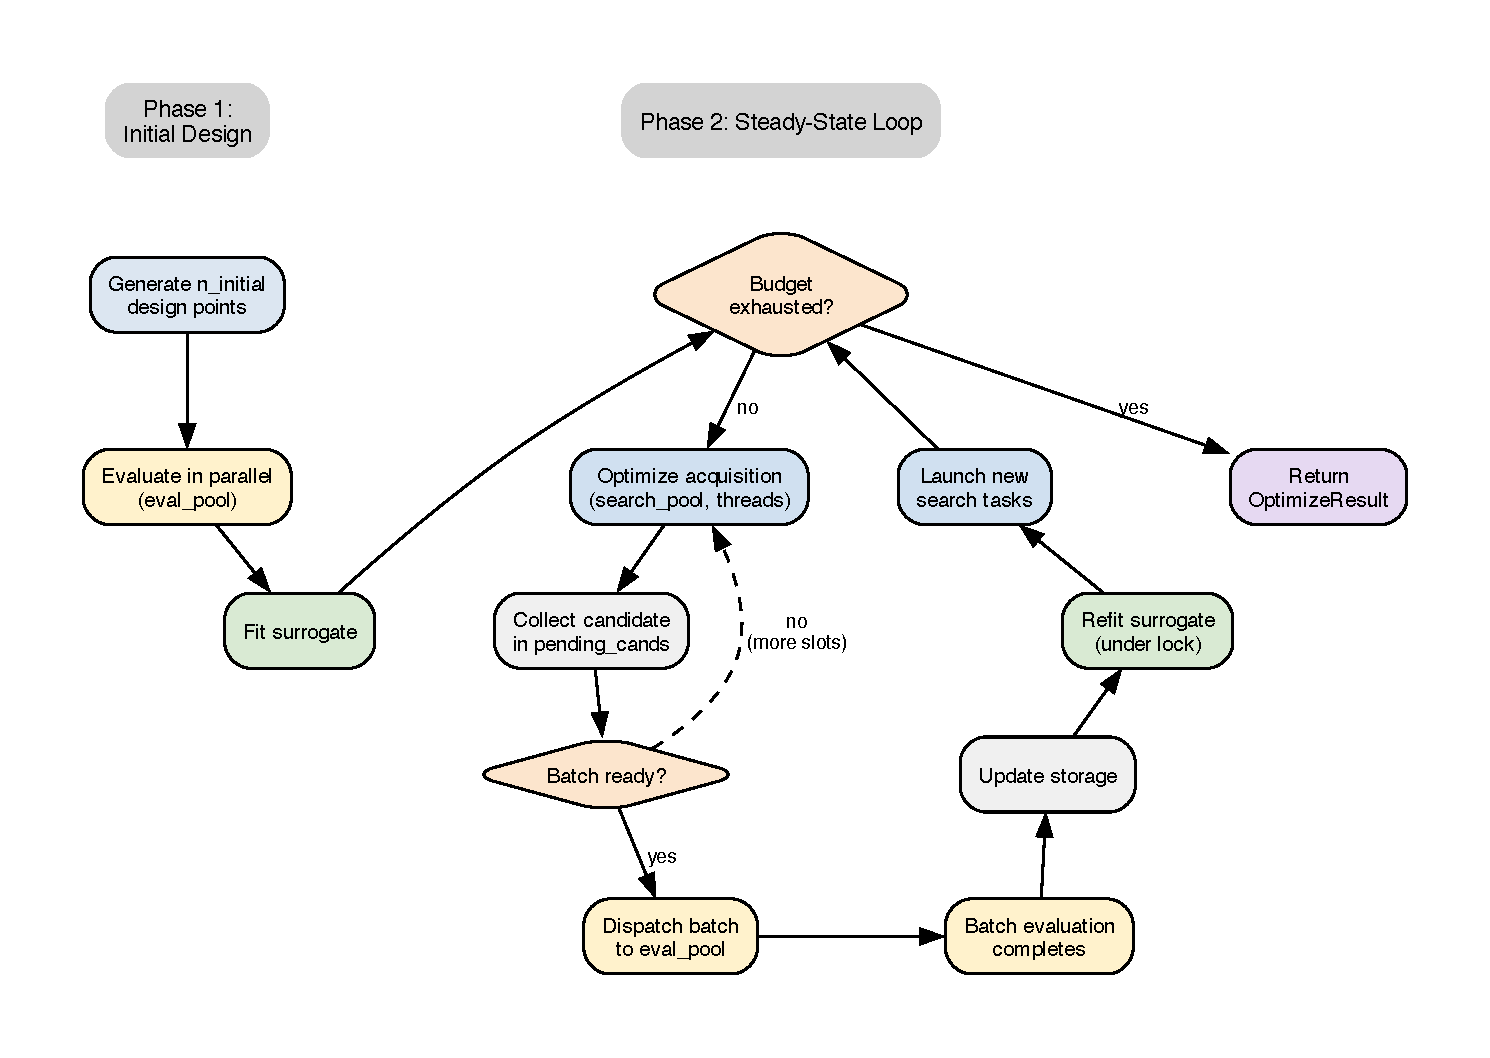
\includegraphics[width=0.95\textwidth]{steady-state.pdf}
\caption{Steady-state parallelization in \texttt{spotoptim}. Phase~1 evaluates the initial design in parallel and fits the first surrogate. Phase~2 overlaps surrogate search (thread pool) with objective evaluation (process or thread pool) in a steady-state loop until the budget is exhausted. Note, \texttt{Optimize acquisition} is the cheap evaluation on the surrogate, the expensive one is performed in the \texttt{eval\_pool} step.}\label{fig-steady-state}
\end{figure*}

On standard CPython builds\footnote{With the Global Interpreter Lock
  (GIL) enabled.}, the evaluation pool uses processes
(\texttt{ProcessPoolExecutor}) so that CPU-bound objective functions
achieve true parallelism, while the search pool uses threads to avoid
serialization overhead for surrogate access. On free-threaded Python
builds\footnote{Python Enhancement Proposal 703, \texttt{python3.13t}.},
both pools use threads, eliminating \texttt{dill} serialization entirely
and reducing dispatch latency. The runtime detects the GIL state
automatically via \texttt{is\_gil\_disabled()} and selects the
appropriate executor. The following example runs a parallel optimization
with four workers:

\begin{Shaded}
\begin{Highlighting}[]
\ImportTok{from}\NormalTok{ spotoptim }\ImportTok{import}\NormalTok{ SpotOptim}
\ImportTok{from}\NormalTok{ spotoptim.function }\ImportTok{import}\NormalTok{ sphere}

\NormalTok{opt }\OperatorTok{=}\NormalTok{ SpotOptim(}
\NormalTok{    fun}\OperatorTok{=}\NormalTok{sphere,}
\NormalTok{    bounds}\OperatorTok{=}\NormalTok{[(}\OperatorTok{{-}}\DecValTok{5}\NormalTok{, }\DecValTok{5}\NormalTok{), (}\OperatorTok{{-}}\DecValTok{5}\NormalTok{, }\DecValTok{5}\NormalTok{)],}
\NormalTok{    max\_iter}\OperatorTok{=}\DecValTok{50}\NormalTok{,}
\NormalTok{    n\_initial}\OperatorTok{=}\DecValTok{10}\NormalTok{,}
\NormalTok{    seed}\OperatorTok{=}\DecValTok{0}\NormalTok{,}
\NormalTok{    n\_jobs}\OperatorTok{=}\DecValTok{4}\NormalTok{,           }\CommentTok{\# parallel workers}
\NormalTok{    eval\_batch\_size}\OperatorTok{=}\DecValTok{2}\NormalTok{,  }\CommentTok{\# batch size}
\NormalTok{)}
\NormalTok{result }\OperatorTok{=}\NormalTok{ opt.optimize()}

\BuiltInTok{print}\NormalTok{(}\SpecialStringTok{f"Best value: }\SpecialCharTok{\{}\NormalTok{result}\SpecialCharTok{.}\NormalTok{fun}\SpecialCharTok{:.6f\}}\SpecialStringTok{"}\NormalTok{)}
\BuiltInTok{print}\NormalTok{(}\SpecialStringTok{f"Total evaluations: }\SpecialCharTok{\{}\NormalTok{result}\SpecialCharTok{.}\NormalTok{nfev}\SpecialCharTok{\}}\SpecialStringTok{"}\NormalTok{)}
\end{Highlighting}
\end{Shaded}

\begin{verbatim}
Best value: 0.000000
Total evaluations: 50
\end{verbatim}

For noisy objective functions, \texttt{spotoptim} supports repeated
evaluations at each design point. The surrogate is fitted on the mean
values across repeats, reducing the influence of noise. When the noise
level varies across the search space, OCBA can be enabled through the
\texttt{ocba\_delta} parameter (Chen 2010). OCBA allocates additional
evaluation budget to the most promising and most uncertain designs,
following the theory developed by Bartz-Beielstein and Friese (2011) and
Bartz-Beielstein et al. (2011). This combination of repeated evaluations
and adaptive budget allocation provides a principled approach to noisy
optimization that is unique among the frameworks discussed in
Section~\ref{sec-related}.

When the optimizer stalls, automatic restarts can help escape local
minima. \texttt{spotoptim} tracks a rolling success rate that measures
the fraction of recent evaluations that improved upon the incumbent best
value. A sliding window of size \texttt{window\_size} records whether
each sequential evaluation achieved a new best; the success rate is the
number of successes divided by the window length. By default
\texttt{window\_size} is set to \texttt{restart\_after\_n} (or 100 if
\texttt{restart\_after\_n} is also unset), so the success rate reflects
performance over the full restart horizon. When no improvement has
occurred for a full window, the success rate drops to zero, signalling
stagnation. The \texttt{restart\_after\_n} parameter (default 100)
specifies how many consecutive iterations with a zero success rate must
elapse before a restart is triggered. Upon restart, the optimizer
generates a fresh initial design and re-initializes the surrogate. If
\texttt{restart\_inject\_best} is \texttt{True} (the default), the best
solution found so far is injected into the new initial design,
preserving accumulated knowledge while allowing the surrogate to explore
a different region of the search space. The following example shows how
to configure the success-rate-based restart mechanism:

\begin{Shaded}
\begin{Highlighting}[]
\ImportTok{from}\NormalTok{ spotoptim }\ImportTok{import}\NormalTok{ SpotOptim}
\ImportTok{from}\NormalTok{ spotoptim.function }\ImportTok{import}\NormalTok{ sphere}

\NormalTok{opt }\OperatorTok{=}\NormalTok{ SpotOptim(}
\NormalTok{    fun}\OperatorTok{=}\NormalTok{sphere,}
\NormalTok{    bounds}\OperatorTok{=}\NormalTok{[(}\OperatorTok{{-}}\DecValTok{5}\NormalTok{, }\DecValTok{5}\NormalTok{), (}\OperatorTok{{-}}\DecValTok{5}\NormalTok{, }\DecValTok{5}\NormalTok{)],}
\NormalTok{    max\_iter}\OperatorTok{=}\DecValTok{20}\NormalTok{,}
\NormalTok{    n\_initial}\OperatorTok{=}\DecValTok{10}\NormalTok{,}
\NormalTok{    seed}\OperatorTok{=}\DecValTok{42}\NormalTok{,}
\NormalTok{    window\_size}\OperatorTok{=}\DecValTok{5}\NormalTok{,}
\NormalTok{    restart\_after\_n}\OperatorTok{=}\DecValTok{10}\NormalTok{,}
\NormalTok{    restart\_inject\_best}\OperatorTok{=}\VariableTok{True}\NormalTok{,}
\NormalTok{    verbose}\OperatorTok{=}\VariableTok{False}\NormalTok{,}
\NormalTok{)}
\NormalTok{result }\OperatorTok{=}\NormalTok{ opt.optimize()}

\BuiltInTok{print}\NormalTok{(}\SpecialStringTok{f"Success rate: }\SpecialCharTok{\{}\NormalTok{opt}\SpecialCharTok{.}\NormalTok{success\_rate}\SpecialCharTok{:.2f\}}\SpecialStringTok{"}\NormalTok{)}
\BuiltInTok{print}\NormalTok{(}\SpecialStringTok{f"Best value: }\SpecialCharTok{\{}\NormalTok{result}\SpecialCharTok{.}\NormalTok{fun}\SpecialCharTok{:.6f\}}\SpecialStringTok{"}\NormalTok{)}
\BuiltInTok{print}\NormalTok{(}\SpecialStringTok{f"Evaluations: }\SpecialCharTok{\{}\NormalTok{result}\SpecialCharTok{.}\NormalTok{nfev}\SpecialCharTok{\}}\SpecialStringTok{"}\NormalTok{)}
\end{Highlighting}
\end{Shaded}

\begin{verbatim}
Success rate: 0.40
Best value: 0.000000
Evaluations: 20
\end{verbatim}

A small \texttt{window\_size} makes the success rate sensitive to short
bursts of improvement, while a larger window smooths out isolated lucky
evaluations. A low \texttt{restart\_after\_n} triggers frequent
restarts, which favours exploration over exploitation; a high value
allows the optimizer to persist longer in a region before restarting.
The success rate is also available programmatically via the
\texttt{success\_rate} attribute, enabling custom termination logic or
logging.

\section{Modules}\label{sec-modules}

The \texttt{spotoptim} codebase is organized into focused modules
(subpackages), each responsible for a specific aspect of the
optimization workflow. Figure\textasciitilde{}\ref{fig-dirtree} shows
the top-level directory structure. This section describes each module,
its purpose, and its key components. Key abbreviations used in the
figure and throughout this section include multi-layer perceptron (MLP)
and principal component analysis (PCA). All modules are imported from
the top-level \texttt{spotoptim} namespace or from the corresponding
subpackage.

\begin{figure*}[ht]
\dirtree{%
.1 src/spotoptim/.
.2 SpotOptim.py\DTcomment{Core optimizer}.
.2 core/\DTcomment{Protocol, storage, experiment control}.
.2 optimizer/\DTcomment{Acquisition, steady-state, scipy wrapper}.
.2 surrogate/\DTcomment{Kriging, MLP surrogate, Nystroem}.
.2 nn/\DTcomment{PyTorch MLP, LinearRegressor}.
.2 function/\DTcomment{Objective functions (single-/multi-objective, remote, torch)}.
.2 sampling/\DTcomment{LHS, Sobol, grid, clustered designs}.
.2 reporting/\DTcomment{Results extraction, analysis utilities}.
.2 plot/\DTcomment{Surrogate visualization, contour, multi-objective plots}.
.2 utils/\DTcomment{Boundaries, transforms, PCA, OCBA, TensorBoard, parallel}.
.2 mo/\DTcomment{Multi-objective: Morris--Mitchell, Pareto front}.
.2 hyperparameters/\DTcomment{Parameter set management for neural network tuning}.
.2 data/\DTcomment{Dataset loaders (e.g., DiabetesDataset)}.
.2 inspection/\DTcomment{Model/surrogate inspection}.
.2 factor\_analyzer/\DTcomment{Factor analysis}.
.2 eda/\DTcomment{Exploratory data analysis}.
.2 tricands/\DTcomment{Triangulation-based candidate generation}.
}
\caption{Top-level directory structure of the \texttt{spotoptim} package.}\label{fig-dirtree}
\end{figure*}

\subsection{The SpotOptim Class}\label{sec-spotoptim-class}

The \texttt{SpotOptim} class in \texttt{spotoptim.SpotOptim} is the
central orchestrator. Its constructor accepts the objective function,
bounds, and a comprehensive set of configuration parameters that control
every aspect of the optimization: the surrogate model, acquisition
function and optimizer, variable types and transformations, evaluation
budget, noise handling, restart policy, and parallelism. All parameters
are stored in a \texttt{SpotOptimConfig} dataclass and can be accessed
as attributes of the optimizer instance. The most commonly used
constructor parameters are \texttt{fun} (the objective function),
\texttt{bounds} (a list of lower/upper tuples), \texttt{max\_iter}
(total evaluation budget including the initial design),
\texttt{n\_initial} (number of initial design points),
\texttt{surrogate} (default: \texttt{Kriging(method="regression")}),
\texttt{acquisition} (\texttt{"y"}, \texttt{"ei"}, or \texttt{"pi"}),
\texttt{var\_type} (list of \texttt{"float"}, \texttt{"int"},
\texttt{"factor"}), and \texttt{seed} (for reproducibility). The
\texttt{optimize()} method executes the algorithm described in
Section~\ref{sec-algorithm} and returns a
\texttt{scipy.optimize.OptimizeResult} with fields \texttt{x} (best
point), \texttt{fun} (best objective value), \texttt{nfev} (total
evaluations), \texttt{nit} (sequential iterations), \texttt{success},
and \texttt{message}. The full evaluated data are available as
\texttt{result.X} and \texttt{result.y}, allowing post-hoc analysis
without re-running the optimization.

Variable transformations can be applied through the \texttt{var\_trans}
parameter. For example, \texttt{var\_trans={[}"log10",\ None{]}}
optimizes the first variable in \(\log_{10}\) space internally while
specifying bounds in natural scale, which is useful for parameters that
span several orders of magnitude such as learning rates. The
\texttt{n\_jobs} parameter enables parallel evaluation of multiple
design points using joblib, and \texttt{eval\_batch\_size} controls how
many points are evaluated in each parallel batch.

\subsection{Core Infrastructure}\label{sec-core}

The \texttt{core} subpackage provides foundational components.
\texttt{SpotOptimProtocol} (defined in \texttt{core/protocol.py}) is a
structural typing protocol (PEP 544) that declares the interface
extracted modules expect from the optimizer. Modules such as
\texttt{optimizer.steady\_state} and \texttt{reporting.analysis} accept
any object matching this protocol rather than importing the concrete
\texttt{SpotOptim} class, avoiding circular imports and facilitating
independent testing. The \texttt{core.storage} module manages the
optimizer's internal data arrays through functions like
\texttt{init\_storage()} and \texttt{update\_storage()}, which handle
appending new evaluation results, updating running statistics, and
tracking the best solution found so far. \texttt{ExperimentControl} is a
dataclass that bundles dataset, model class, hyperparameters, device
settings, and training parameters into a single object for PyTorch-based
experiment workflows.

\subsection{Surrogate Models}\label{sec-surrogate}

The \texttt{surrogate} subpackage contains three surrogate
implementations. \texttt{Kriging} is the default and models the
objective as a Gaussian process with a Gaussian (squared-exponential)
kernel, yielding both a mean prediction \(\mu(\mathbf{x})\) and a
standard deviation \(\sigma(\mathbf{x})\) that is essential for
uncertainty-aware acquisition functions. Its key parameters include
\texttt{method} (see below), \texttt{noise} (regularization term),
\texttt{min\_theta} and \texttt{max\_theta} (bounds for log-scaled
kernel hyperparameters), and \texttt{seed}; a call to
\texttt{predict(X,\ return\_std=True)} returns both outputs.

The kernel hyperparameters \(\boldsymbol{\theta}\) are estimated by
maximizing the concentrated log-likelihood using differential evolution.
Following Forrester et al. (2008),\footnote{Specifically, Section 2.4
  ``Kriging'' for the core predictor and likelihood, and Section 6
  ``Surrogate Modeling of Noisy Data'' for the \texttt{"regression"} and
  \texttt{"reinterpolation"} methods. The Python code is based on
  \texttt{likelihood.m} (concentrated log-likelihood) and
  \texttt{pred.m} (prediction and error estimation) from the book's
  codebase.} three fitting modes are available via the \texttt{method}
argument: \texttt{"regression"} (default) fits a generalized
least-squares model, \texttt{"interpolation"} passes exactly through the
data points, and \texttt{"reinterpolation"} applies Forrester's
correction for noisy data. The implementation is validated against the
Matlab code of Forrester et al. (2008).

The Kriging implementation in SPO uses flexible kernel functions that
extend naturally to non-continuous parameter spaces. For categorical and
combinatorial variables, appropriate distance or similarity measures
replace the standard Euclidean distance in the correlation function,
enabling the surrogate to model landscapes over discrete, permutation,
or mixed search spaces (Bartz-Beielstein and Zaefferer 2017; Zaefferer
and Bartz-Beielstein 2016). This line of research has produced kernels
for permutation-based problems using tailored distance measures with
automated selection via maximum likelihood estimation (Zaefferer, Stork,
and Bartz-Beielstein 2014; Zaefferer, Stork, Friese, et al. 2014), as
well as kernels for hierarchical and conditional parameter spaces
arising in algorithm configuration (Gentile et al. 2021, 2018).

\begin{Shaded}
\begin{Highlighting}[]
\ImportTok{import}\NormalTok{ numpy }\ImportTok{as}\NormalTok{ np}
\ImportTok{from}\NormalTok{ spotoptim.surrogate }\ImportTok{import}\NormalTok{ Kriging}

\NormalTok{X\_train }\OperatorTok{=}\NormalTok{ np.array([[}\FloatTok{0.0}\NormalTok{], [}\FloatTok{1.0}\NormalTok{], [}\FloatTok{3.0}\NormalTok{], [}\FloatTok{4.0}\NormalTok{]])}
\NormalTok{y\_train }\OperatorTok{=}\NormalTok{ np.array([}\FloatTok{0.0}\NormalTok{, }\FloatTok{1.0}\NormalTok{, }\FloatTok{9.0}\NormalTok{, }\FloatTok{16.0}\NormalTok{])}

\NormalTok{model }\OperatorTok{=}\NormalTok{ Kriging(method}\OperatorTok{=}\StringTok{"regression"}\NormalTok{, seed}\OperatorTok{=}\DecValTok{0}\NormalTok{)}
\NormalTok{model.fit(X\_train, y\_train)}

\NormalTok{X\_test }\OperatorTok{=}\NormalTok{ np.array([[}\FloatTok{0.5}\NormalTok{], [}\FloatTok{2.0}\NormalTok{], [}\FloatTok{3.5}\NormalTok{]])}
\NormalTok{y\_pred, y\_std }\OperatorTok{=}\NormalTok{ model.predict(}
\NormalTok{    X\_test, return\_std}\OperatorTok{=}\VariableTok{True}
\NormalTok{)}
\end{Highlighting}
\end{Shaded}

\texttt{SimpleKriging} is a lightweight alternative for simple
continuous problems where computational speed takes priority over
flexibility. \texttt{MLPSurrogate} uses a multi-layer perceptron (MLP),
which is useful when the response surface is highly non-linear or when
the number of data points exceeds the practical limits of Kriging's
\(\mathcal{O}(n^3)\) fitting cost. Alternatively, a Nystroem
approximation module (\texttt{surrogate/nystroem.py}) provides further
scalability for large datasets. Uncertainty estimates from
\texttt{MLPSurrogate} are obtained by performing multiple forward passes
with dropout enabled and computing the empirical variance across passes.

The surrogate interface follows the scikit-learn estimator convention.
Any model that implements \texttt{fit(X,\ y)} and \texttt{predict(X)}
can be passed as the \texttt{surrogate} argument to \texttt{SpotOptim}.
For acquisition functions that require uncertainty (\texttt{"ei"},
\texttt{"pi"}), the model should additionally support
\texttt{predict(X,\ return\_std=True)}. This makes it straightforward to
use scikit-learn's \texttt{GaussianProcessRegressor} with custom
kernels, or any other regression model, as a drop-in replacement for
Kriging.

Beyond single-surrogate optimization, \texttt{spotoptim} supports
multi-surrogate scheduling. The \texttt{surrogate} parameter accepts a
list of surrogate models together with a \texttt{prob\_surrogate} vector
that specifies the selection probability for each model. At every
surrogate refit step, one model is drawn at random according to these
weights and used for the next acquisition cycle. This introduces
diversity into the search: different surrogate types may fit different
regions of the landscape better, and alternating between them can reduce
the risk of systematic model bias. Each surrogate can also have its own
\texttt{max\_surrogate\_points} budget, passed as a list of the same
length. If \texttt{prob\_surrogate} is omitted, uniform weights are
assigned automatically. The following example combines a Kriging model
(selected with probability 0.7) and a random forest (selected with
probability 0.3):

\begin{Shaded}
\begin{Highlighting}[]
\ImportTok{from}\NormalTok{ spotoptim }\ImportTok{import}\NormalTok{ SpotOptim}
\ImportTok{from}\NormalTok{ spotoptim.surrogate }\ImportTok{import}\NormalTok{ Kriging}
\ImportTok{from}\NormalTok{ sklearn.ensemble }\ImportTok{import}\NormalTok{ RandomForestRegressor}
\ImportTok{from}\NormalTok{ spotoptim.function }\ImportTok{import}\NormalTok{ sphere}

\NormalTok{kriging }\OperatorTok{=}\NormalTok{ Kriging(method}\OperatorTok{=}\StringTok{"regression"}\NormalTok{, seed}\OperatorTok{=}\DecValTok{0}\NormalTok{)}
\NormalTok{rf }\OperatorTok{=}\NormalTok{ RandomForestRegressor(}
\NormalTok{    n\_estimators}\OperatorTok{=}\DecValTok{50}\NormalTok{, random\_state}\OperatorTok{=}\DecValTok{0}
\NormalTok{)}

\NormalTok{opt }\OperatorTok{=}\NormalTok{ SpotOptim(}
\NormalTok{    fun}\OperatorTok{=}\NormalTok{sphere,}
\NormalTok{    bounds}\OperatorTok{=}\NormalTok{[(}\OperatorTok{{-}}\DecValTok{5}\NormalTok{, }\DecValTok{5}\NormalTok{), (}\OperatorTok{{-}}\DecValTok{5}\NormalTok{, }\DecValTok{5}\NormalTok{)],}
\NormalTok{    max\_iter}\OperatorTok{=}\DecValTok{30}\NormalTok{,}
\NormalTok{    n\_initial}\OperatorTok{=}\DecValTok{10}\NormalTok{,}
\NormalTok{    seed}\OperatorTok{=}\DecValTok{0}\NormalTok{,}
\NormalTok{    surrogate}\OperatorTok{=}\NormalTok{[kriging, rf],}
\NormalTok{    prob\_surrogate}\OperatorTok{=}\NormalTok{[}\FloatTok{0.7}\NormalTok{, }\FloatTok{0.3}\NormalTok{],}
\NormalTok{    max\_surrogate\_points}\OperatorTok{=}\NormalTok{[}\VariableTok{None}\NormalTok{, }\DecValTok{50}\NormalTok{],}
    \CommentTok{\# no cap for Kriging, 50 for RF}
\NormalTok{)}
\NormalTok{result }\OperatorTok{=}\NormalTok{ opt.optimize()}

\BuiltInTok{print}\NormalTok{(}\SpecialStringTok{f"Best value: }\SpecialCharTok{\{}\NormalTok{result}\SpecialCharTok{.}\NormalTok{fun}\SpecialCharTok{:.6f\}}\SpecialStringTok{"}\NormalTok{)}
\end{Highlighting}
\end{Shaded}

\begin{verbatim}
Best value: 0.000000
\end{verbatim}

\subsection{Acquisition and Infill}\label{sec-optimizer}

The \texttt{optimizer} subpackage implements the acquisition functions,
their optimizers as well as infill-point selection.

\textbf{Acquisition functions.} The \texttt{acquisition\_function}
parameter selects which criterion is used to propose the next evaluation
point. Three options are available. \emph{Predicted value}
(\texttt{"y"}) selects the point where the surrogate predicts the lowest
(or highest, for maximization) objective value. This is the simplest
strategy and amounts to pure exploitation of the current model. It is
computationally cheap but can become trapped in local minima because it
does not account for surrogate uncertainty. \emph{Expected Improvement}
(\texttt{"ei"}) balances exploitation and exploration by weighting the
predicted improvement over the current best value \(y_{\min}\) against
the surrogate's predictive uncertainty \(\sigma(\mathbf{x})\). The EI
formula (Equation~\ref{eq-ei}) was introduced in
Section~\ref{sec-examples}; points with high predicted quality \emph{or}
high uncertainty receive large EI values, which encourages the optimizer
to explore under-sampled regions. \emph{Probability of Improvement}
(\texttt{"pi"}) selects the point with the highest probability of
producing an objective value below the current best \(y_{\min}\).
Probability of Improvement tends to be more exploitative than EI,
because it only measures the probability of any improvement, not its
expected magnitude.

\textbf{Acquisition optimizers.} The \texttt{acquisition\_optimizer}
parameter determines how the acquisition function is maximized over the
search space. Differential evolution (the default) performs a global
search and is robust across a wide range of problem structures (Storn
1996). The triangulation candidates approach implements the approach
developed by Gramacy et al. (2022), generating candidate points
geometrically from the Delaunay triangulation of existing evaluations,
producing both interior candidates at simplex centroids and fringe
candidates that extend toward the search space boundary, see also
Section~\ref{sec-tricands}. The hybrid \texttt{de\_tricands} mode, which
is still experimental and has not been analyzed so far, alternates
between the two methods with probability controlled by
\texttt{prob\_de\_tricands}. Standard scipy minimizers are also
supported for local refinement.

\textbf{Infill points.} Multiple infill points can be proposed per
iteration by setting \texttt{n\_infill\_points}, which is useful for
batch-parallel evaluation. When the acquisition optimizer fails to find
a valid new point (for example due to a flat surrogate surface), a
random fallback point is generated within bounds. For problems with many
evaluation points, the \texttt{max\_surrogate\_points} parameter limits
the number of data points used for surrogate fitting, keeping
computational cost manageable as the number of evaluations grows. Points
are selected using K-means clustering with either a space-filling
criterion (\texttt{"distant"}) or a quality-based criterion
(\texttt{"best"}).

\subsection{Neural Network Models}\label{sec-nn}

The \texttt{nn} subpackage provides two PyTorch modules designed for use
as objective functions and surrogates in hyperparameter tuning
workflows. The \texttt{MLP} class is a \texttt{torch.nn.Sequential}
subclass with configurable width, depth, activation, and dropout. The
architecture can be specified either explicitly through a
\texttt{hidden\_channels} list or compactly through \texttt{l1} (neurons
per hidden layer) and \texttt{num\_hidden\_layers}, which is the
representation used during hyperparameter tuning.

\begin{Shaded}
\begin{Highlighting}[]
\ImportTok{import}\NormalTok{ torch}
\ImportTok{from}\NormalTok{ spotoptim.nn }\ImportTok{import}\NormalTok{ MLP}

\NormalTok{model }\OperatorTok{=}\NormalTok{ MLP(}
\NormalTok{    in\_channels}\OperatorTok{=}\DecValTok{10}\NormalTok{,}
\NormalTok{    l1}\OperatorTok{=}\DecValTok{64}\NormalTok{,}
\NormalTok{    num\_hidden\_layers}\OperatorTok{=}\DecValTok{2}\NormalTok{,}
\NormalTok{    output\_dim}\OperatorTok{=}\DecValTok{1}\NormalTok{,}
\NormalTok{    dropout}\OperatorTok{=}\FloatTok{0.1}\NormalTok{,}
\NormalTok{)}
\end{Highlighting}
\end{Shaded}

\texttt{LinearRegressor} is a \texttt{torch.nn.Module} for regression
tasks that ranges from pure linear regression (with
\texttt{num\_hidden\_layers=0}) to a deep network with configurable
activation functions. Both classes provide a
\texttt{get\_default\_parameters()} class method that returns a
\texttt{ParameterSet} with sensible bounds for hyperparameter tuning,
and a \texttt{get\_optimizer()} method that maps string names to
\texttt{torch.optim} optimizer classes. Beyond standard PyTorch
optimizers, \texttt{spotoptim} bundles \texttt{AdamWScheduleFree}, a
schedule-free variant of AdamW that does not require a learning-rate
scheduler.

\subsection{Built-in Test Functions}\label{sec-functions}

The \texttt{function} subpackage contains analytical test functions for
benchmarking and testing. All functions accept a 2-D array of shape
\((n, d)\) and return a 1-D array of shape \((n,)\) for single-objective
functions, or \((n, m)\) for multi-objective functions, where \(n\),
\(d\), and \(m\) denote the number of samples, dimensions, and
objectives, respectively.

The single-objective functions include sphere, noisy sphere (sphere with
additive Gaussian noise), Rosenbrock (narrow curved valley, minimum at
\(\mathbf{1}\)), Ackley (multi-modal with many local minima), and
Michalewicz (steep valleys with a tunable steepness parameter).
Engineering benchmark functions include \texttt{wingwt} (wing weight
estimation, 9--10 dimensions from Forrester et al. (2008)),
\texttt{robot\_arm\_hard} (10-link robot arm maze navigation), and
\texttt{lennard\_jones} (atomic cluster potential, 39 dimensions for 13
atoms). Multi-objective functions include the ZDT family (\texttt{zdt1}
through \texttt{zdt6}), DTLZ problems (\texttt{dtlz1}, \texttt{dtlz2}),
Fonseca-Fleming, Schaffer N1, and Kursawe. Custom objective functions
can be defined by the user following the same array convention.

\subsection{Sampling and Experimental Designs}\label{sec-sampling}

The \texttt{sampling.design} module provides space-filling designs for
the initial evaluation phase. The default quasi-Monte Carlo Latin
Hypercube design (\texttt{generate\_qmc\_lhs\_design}) ensures that each
variable's marginal distribution is uniformly covered. Sobol sequences
(\texttt{generate\_sobol\_design}) provide quasi-random low-discrepancy
coverage that is particularly effective in higher dimensions. Regular
grids (\texttt{generate\_grid\_design}) place points at equal intervals;
the actual number of grid points is
\(\lfloor n_\text{design}^{1/d} \rfloor^d\), where \(n_\text{design}\)
is the requested number of points. Uniform random sampling
(\texttt{generate\_uniform\_design}) serves as a baseline, and clustered
designs (\texttt{generate\_clustered\_design}) produce non-uniform
distributions for testing optimizer robustness and generating so-called
``ill-conditioned'' designs.

\begin{Shaded}
\begin{Highlighting}[]
\ImportTok{from}\NormalTok{ spotoptim.sampling.design }\ImportTok{import}\NormalTok{ (}
\NormalTok{    generate\_qmc\_lhs\_design,}
\NormalTok{    generate\_sobol\_design,}
\NormalTok{)}

\NormalTok{bounds }\OperatorTok{=}\NormalTok{ [(}\OperatorTok{{-}}\DecValTok{5}\NormalTok{, }\DecValTok{5}\NormalTok{), (}\OperatorTok{{-}}\DecValTok{5}\NormalTok{, }\DecValTok{5}\NormalTok{)]}
\NormalTok{X\_lhs }\OperatorTok{=}\NormalTok{ generate\_qmc\_lhs\_design(}
\NormalTok{    bounds, n\_design}\OperatorTok{=}\DecValTok{20}\NormalTok{, seed}\OperatorTok{=}\DecValTok{0}
\NormalTok{)}
\NormalTok{X\_sobol }\OperatorTok{=}\NormalTok{ generate\_sobol\_design(}
\NormalTok{    bounds, n\_design}\OperatorTok{=}\DecValTok{32}\NormalTok{, seed}\OperatorTok{=}\DecValTok{0}
\NormalTok{)}
\end{Highlighting}
\end{Shaded}

A pre-computed initial design can be passed to
\texttt{SpotOptim.optimize()} via the \texttt{X0} parameter, allowing
the user to incorporate prior knowledge or to resume an optimization
from a previous set of evaluations.

\subsection{Reporting and Analysis}\label{sec-reporting}

The \texttt{reporting} subpackage extracts and formats optimization
results. \texttt{print\_best} displays the best parameter vector and
objective value in a human-readable format, with factor variables mapped
back to their string labels. \texttt{get\_results\_table} produces a
formatted table showing each variable's name, type, bounds, default
value, and tuned (best) value, with an optional importance score column.
\texttt{get\_design\_table} summarizes the search space before
optimization, listing variable types, bounds, and transformations. For
post-hoc analysis, \texttt{get\_importance} computes a correlation-based
importance score for each variable on a 0--100 scale, and
\texttt{sensitivity\_spearman} reports Spearman rank correlations
between each parameter and the objective value, together with p-values
and significance stars. These tools help identify which hyperparameters
have the strongest influence on performance, guiding subsequent
refinements to the search space.

\subsection{Visualization}\label{sec-plotting}

The \texttt{plot} subpackage provides several visualization functions.
\texttt{plot\_progress} displays the full evaluation history as a
scatter plot with a best-so-far curve overlaid, distinguishing initial
design points from sequential evaluations. \texttt{plot\_surrogate}
renders a 2x2 panel showing the fitted surrogate model for a selected
pair of dimensions: the top row contains 3-D surfaces of predictions and
prediction uncertainty, while the bottom row shows the corresponding
contour plots with evaluated points overlaid. \texttt{simple\_contour}
draws a quick 2-D filled contour of any callable over a rectangular
region, and \texttt{plot\_design\_points} creates a scatter plot of
evaluated points with hidden-dimension aggregation. Multi-objective
visualization is provided through \texttt{mo\_pareto\_optx\_plot}, which
shows Pareto-optimal points in the input space, and
\texttt{mo\_xy\_contour} and \texttt{mo\_xy\_surface} for
surrogate-based objective-space visualization. The following examples
use the sphere function optimized over \([-5, 5]^2\) with 25 iterations.
Figure~\ref{fig-progress} shows a typical progress plot. The initial
design points appear as grey dots in a shaded background region;
sequential evaluations are connected by a line, and the red curve traces
the best objective value found so far.

\begin{Shaded}
\begin{Highlighting}[]
\ImportTok{from}\NormalTok{ spotoptim }\ImportTok{import}\NormalTok{ SpotOptim}
\ImportTok{from}\NormalTok{ spotoptim.function }\ImportTok{import}\NormalTok{ sphere}
\ImportTok{from}\NormalTok{ spotoptim.plot.visualization }\ImportTok{import}\NormalTok{ (}
\NormalTok{    plot\_progress}
\NormalTok{)}

\NormalTok{opt }\OperatorTok{=}\NormalTok{ SpotOptim(}
\NormalTok{    fun}\OperatorTok{=}\NormalTok{sphere,}
\NormalTok{    bounds}\OperatorTok{=}\NormalTok{[(}\OperatorTok{{-}}\DecValTok{5}\NormalTok{, }\DecValTok{5}\NormalTok{), (}\OperatorTok{{-}}\DecValTok{5}\NormalTok{, }\DecValTok{5}\NormalTok{)],}
\NormalTok{    max\_iter}\OperatorTok{=}\DecValTok{25}\NormalTok{,}
\NormalTok{    n\_initial}\OperatorTok{=}\DecValTok{10}\NormalTok{,}
\NormalTok{    seed}\OperatorTok{=}\DecValTok{0}\NormalTok{,}
\NormalTok{)}
\NormalTok{result }\OperatorTok{=}\NormalTok{ opt.optimize()}
\NormalTok{plot\_progress(opt, show}\OperatorTok{=}\VariableTok{False}\NormalTok{, figsize}\OperatorTok{=}\NormalTok{(}\DecValTok{6}\NormalTok{, }\DecValTok{4}\NormalTok{), log\_y}\OperatorTok{=}\VariableTok{True}\NormalTok{)}
\end{Highlighting}
\end{Shaded}

\begin{figure}[H]

\centering{

\pandocbounded{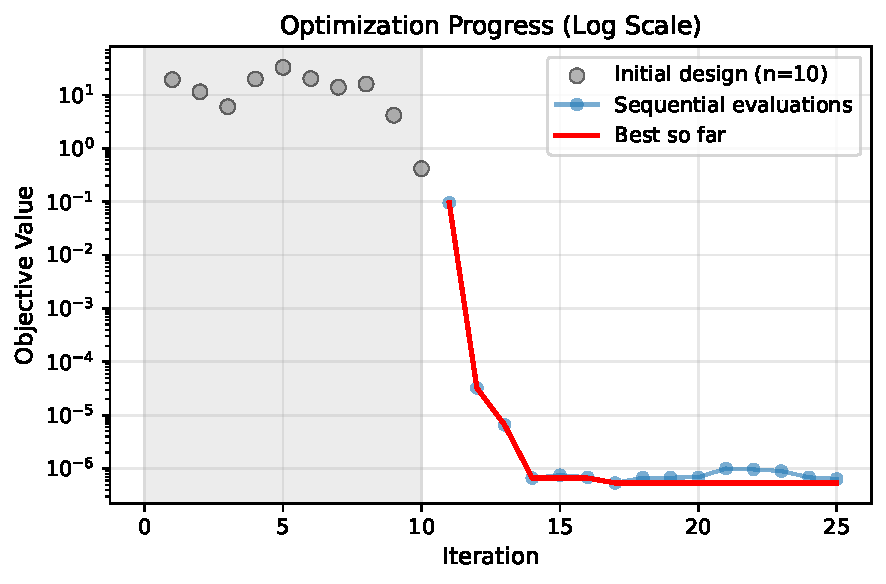
\includegraphics[keepaspectratio]{fig-progress-output-1.pdf}}

}

\caption{\label{fig-progress}Optimization progress for the sphere
function. Grey dots mark the initial Latin Hypercube design; subsequent
evaluations are connected by a line. The red curve shows the best
objective value found so far.}

\end{figure}%

Figure~\ref{fig-surrogate} shows the surrogate model fitted after
optimization. The top row displays 3-D surfaces of the predicted
objective value and the prediction uncertainty; the bottom row shows the
corresponding contour maps with the evaluated points overlaid as red
dots.

\begin{Shaded}
\begin{Highlighting}[]
\ImportTok{from}\NormalTok{ spotoptim.plot.visualization }\ImportTok{import}\NormalTok{ (}
\NormalTok{    plot\_surrogate}
\NormalTok{)}
\NormalTok{plot\_surrogate(opt, i}\OperatorTok{=}\DecValTok{0}\NormalTok{, j}\OperatorTok{=}\DecValTok{1}\NormalTok{, show}\OperatorTok{=}\VariableTok{False}\NormalTok{)}
\end{Highlighting}
\end{Shaded}

\begin{figure}[H]

\centering{

\pandocbounded{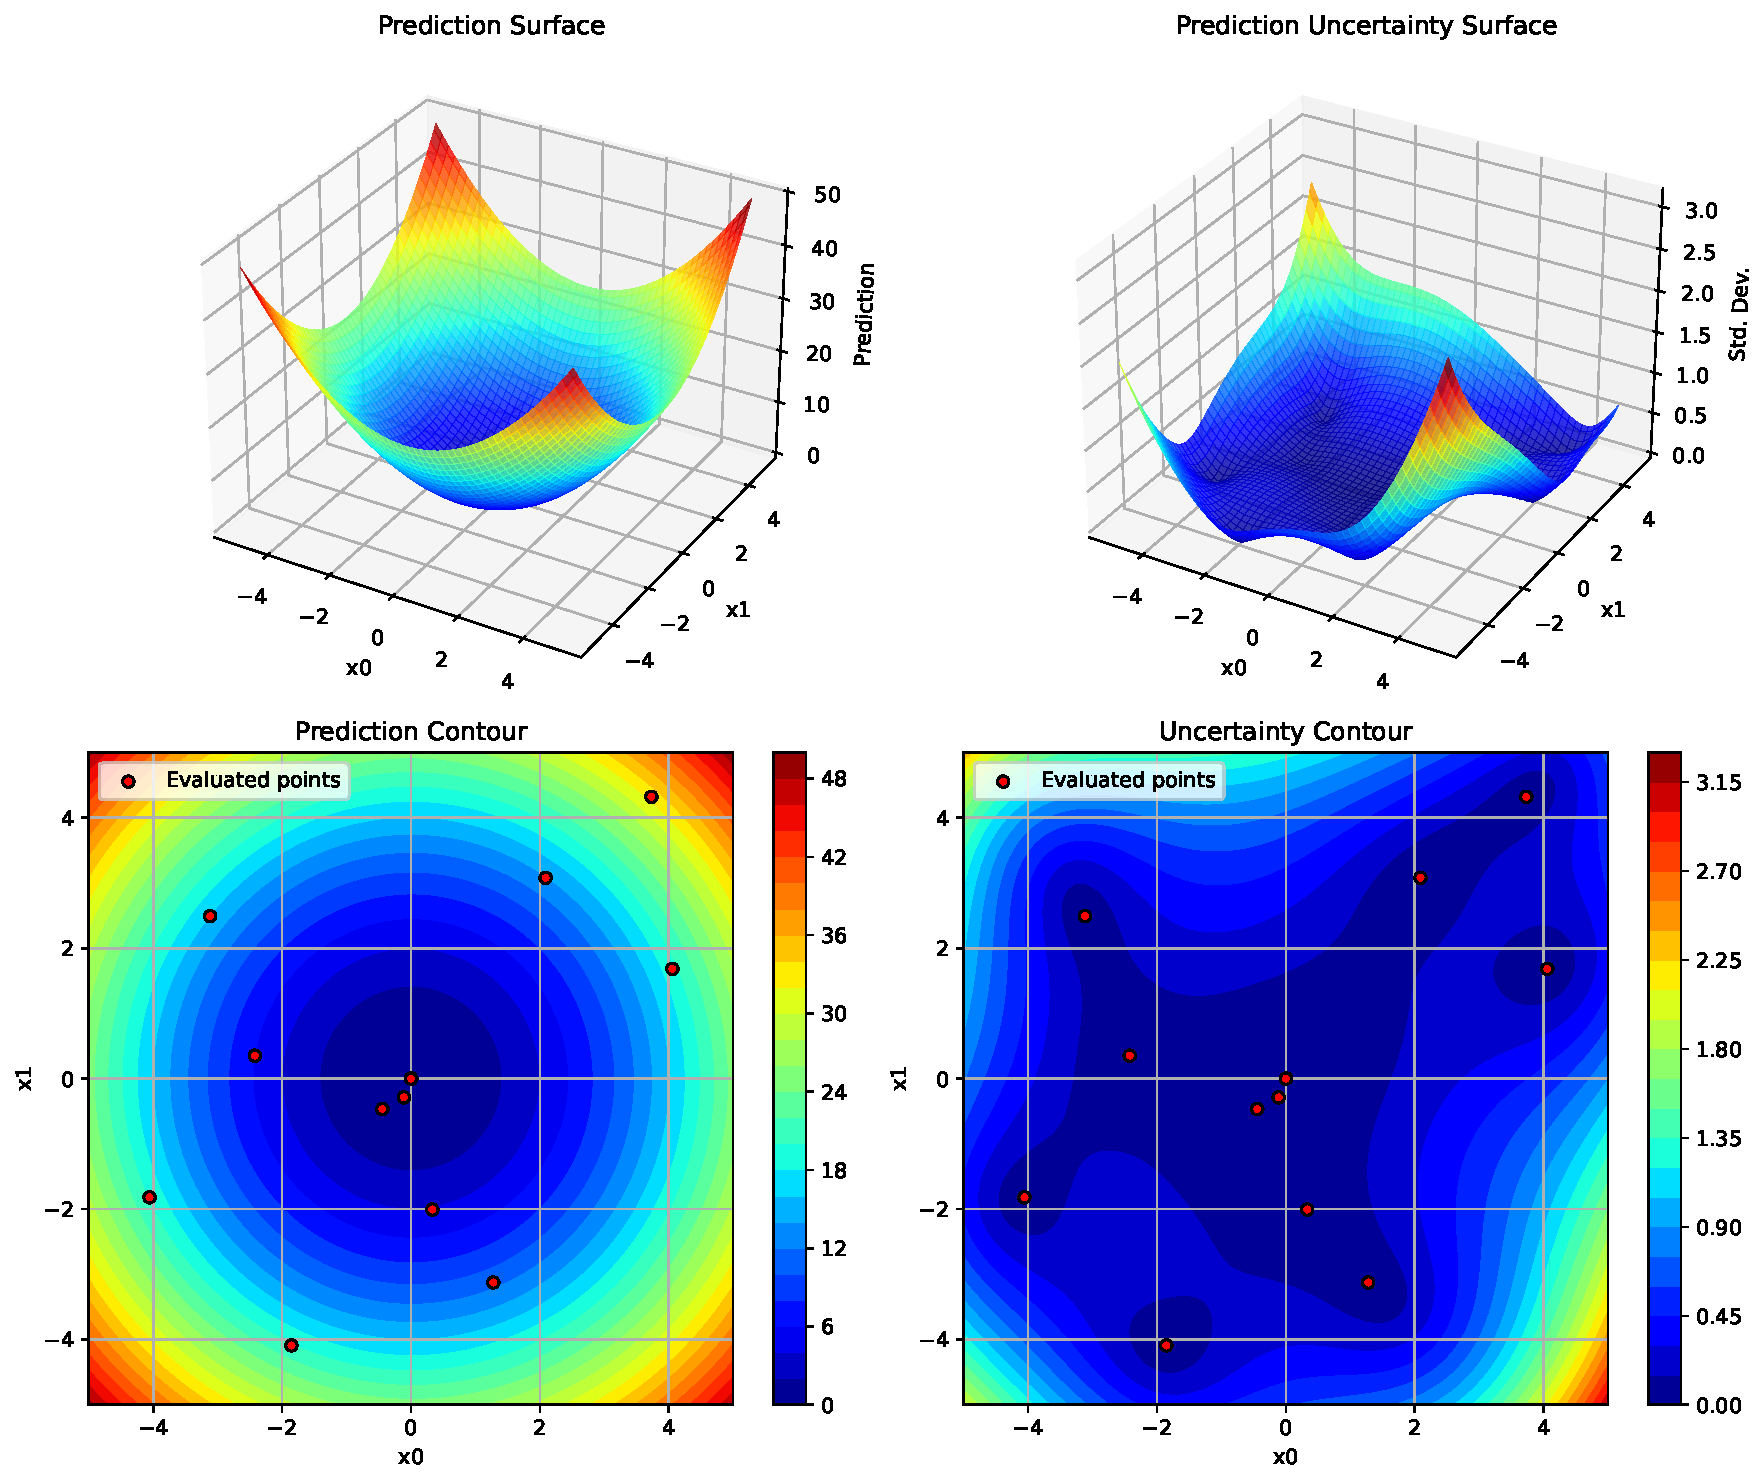
\includegraphics[keepaspectratio]{fig-surrogate-output-1.pdf}}

}

\caption{\label{fig-surrogate}Surrogate model for dimensions \(x_0\) and
\(x_1\). Top row: 3-D surfaces of predictions (left) and prediction
uncertainty (right). Bottom row: contour plots with evaluated points
overlaid.}

\end{figure}%

Figure~\ref{fig-contour} illustrates \texttt{simple\_contour} applied to
the Rosenbrock function. The function accepts any callable that maps a
\((1, 2)\) array to a scalar, making it convenient for quick inspection
of objective landscapes independently of an optimization run.

\begin{Shaded}
\begin{Highlighting}[]
\ImportTok{from}\NormalTok{ spotoptim.function }\ImportTok{import}\NormalTok{ rosenbrock}
\ImportTok{from}\NormalTok{ spotoptim.plot.contour }\ImportTok{import}\NormalTok{ (}
\NormalTok{    simple\_contour}
\NormalTok{)}
\NormalTok{simple\_contour(rosenbrock,}
\NormalTok{    min\_x}\OperatorTok{={-}}\DecValTok{2}\NormalTok{, max\_x}\OperatorTok{=}\DecValTok{2}\NormalTok{, min\_y}\OperatorTok{={-}}\DecValTok{1}\NormalTok{, max\_y}\OperatorTok{=}\DecValTok{3}\NormalTok{,}
\NormalTok{    n\_levels}\OperatorTok{=}\DecValTok{30}\NormalTok{)}
\end{Highlighting}
\end{Shaded}

\begin{figure}[H]

\centering{

\pandocbounded{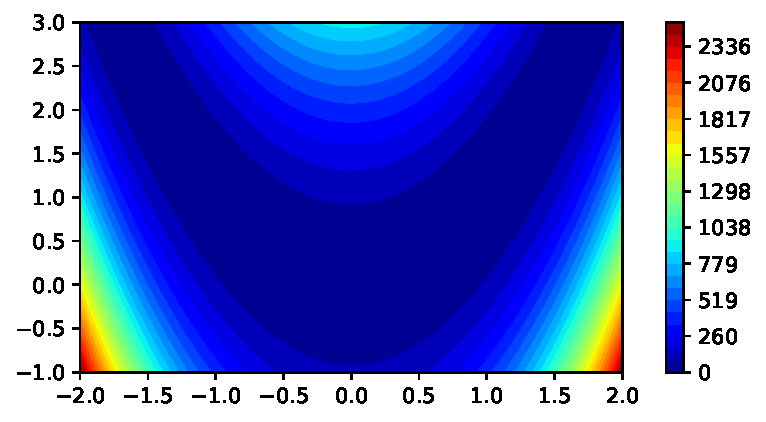
\includegraphics[keepaspectratio]{fig-contour-output-1.pdf}}

}

\caption{\label{fig-contour}Filled contour plot of the Rosenbrock
function over \([-2, 2] \times [-1, 3]\).}

\end{figure}%

For multi-objective problems, \texttt{mo\_pareto\_optx\_plot} visualizes
Pareto-optimal points in the input space. The surrogate-based
visualization functions \texttt{mo\_xy\_contour} and
\texttt{mo\_xy\_surface} generate contour and surface plots for each
objective from fitted surrogate models. Figure~\ref{fig-mo-contour}
shows the contour view for two Kriging surrogates fitted to the
Fonseca--Fleming objectives.

\begin{Shaded}
\begin{Highlighting}[]
\ImportTok{import}\NormalTok{ numpy }\ImportTok{as}\NormalTok{ np}
\ImportTok{from}\NormalTok{ spotoptim.function }\ImportTok{import}\NormalTok{ fonseca\_fleming}
\ImportTok{from}\NormalTok{ spotoptim.surrogate }\ImportTok{import}\NormalTok{ Kriging}
\ImportTok{from}\NormalTok{ spotoptim.mo.pareto }\ImportTok{import}\NormalTok{ mo\_xy\_contour}

\NormalTok{rng }\OperatorTok{=}\NormalTok{ np.random.default\_rng(}\DecValTok{0}\NormalTok{)}
\NormalTok{X\_mo }\OperatorTok{=}\NormalTok{ rng.uniform(}\OperatorTok{{-}}\DecValTok{4}\NormalTok{, }\DecValTok{4}\NormalTok{, size}\OperatorTok{=}\NormalTok{(}\DecValTok{50}\NormalTok{, }\DecValTok{2}\NormalTok{))}
\NormalTok{Y\_mo }\OperatorTok{=}\NormalTok{ fonseca\_fleming(X\_mo)}

\NormalTok{m1 }\OperatorTok{=}\NormalTok{ Kriging()}
\NormalTok{m1.fit(X\_mo, Y\_mo[:, }\DecValTok{0}\NormalTok{])}
\NormalTok{m2 }\OperatorTok{=}\NormalTok{ Kriging()}
\NormalTok{m2.fit(X\_mo, Y\_mo[:, }\DecValTok{1}\NormalTok{])}
\NormalTok{mo\_xy\_contour(}
\NormalTok{    [m1, m2],}
\NormalTok{    bounds}\OperatorTok{=}\NormalTok{[(}\OperatorTok{{-}}\DecValTok{4}\NormalTok{, }\DecValTok{4}\NormalTok{), (}\OperatorTok{{-}}\DecValTok{4}\NormalTok{, }\DecValTok{4}\NormalTok{)],}
\NormalTok{    target\_names}\OperatorTok{=}\NormalTok{[}\StringTok{"f1"}\NormalTok{, }\StringTok{"f2"}\NormalTok{],}
\NormalTok{    feature\_names}\OperatorTok{=}\NormalTok{[}\StringTok{"x0"}\NormalTok{, }\StringTok{"x1"}\NormalTok{],}
\NormalTok{    resolution}\OperatorTok{=}\DecValTok{50}\NormalTok{,}
\NormalTok{)}
\end{Highlighting}
\end{Shaded}

\begin{figure}[H]

\centering{

\pandocbounded{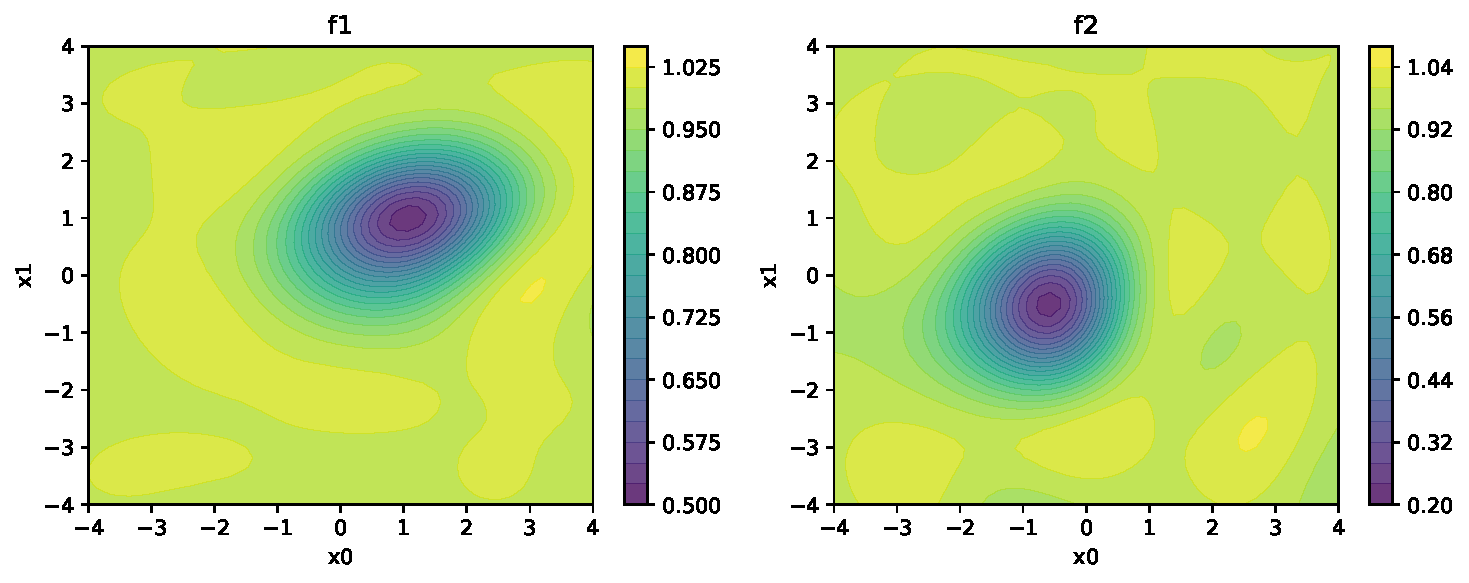
\includegraphics[keepaspectratio]{fig-mo-contour-output-1.pdf}}

}

\caption{\label{fig-mo-contour}Surrogate contour plots for both
Fonseca--Fleming objectives, fitted from 50 random evaluations.}

\end{figure}%

\subsection{Utilities}\label{sec-utils}

The \texttt{utils} subpackage collects helper functions that support the
optimization loop and post-hoc analysis. \texttt{get\_boundaries}
computes column-wise minima and maxima, and
\texttt{map\_to\_original\_scale} transforms points from the \([0, 1]\)
unit hypercube back to the original variable ranges. PCA utilities
(\texttt{get\_pca}, \texttt{get\_pca\_topk}) perform PCA on evaluation
data and identify the features with the strongest loadings on the first
two components.

OCBA functions (\texttt{get\_ocba}, \texttt{get\_ranks}) implement the
OCBA algorithm for noisy optimization (Bartz-Beielstein and Friese
2011). Given current sample means, variances, and an incremental budget,
\texttt{get\_ocba} returns an allocation vector that concentrates
additional evaluations on the most promising and most uncertain designs.
\texttt{TorchStandardScaler} standardizes PyTorch tensors to zero mean
and unit variance, analogous to scikit-learn's \texttt{StandardScaler}.
The \texttt{is\_gil\_disabled} function checks whether the Python
interpreter is a free-threaded build (PEP 703), which \texttt{spotoptim}
uses internally to decide whether thread-based parallelism is safe for
objective evaluation.

The TensorBoard integration (\texttt{utils/tensorboard.py}) provides
real-time monitoring of the optimization process. Setting
\texttt{tensorboard\_log=True} in the \texttt{SpotOptim} constructor
activates logging: at each iteration, the module writes scalar metrics
(current best objective value, last evaluation, success rate) and the
coordinates of the best design point to a TensorBoard event file. For
noisy optimization with repeated evaluations, additional statistics are
logged, including the best mean objective value and the variance at the
best design. Each evaluated hyperparameter configuration is also logged
via \texttt{add\_hparams}, which populates TensorBoard's HParams
dashboard and enables interactive comparison of configurations across
runs. The log directory defaults to
\texttt{runs/spotoptim\_YYYYMMDD\_HHMMSS} but can be customized via the
\texttt{tensorboard\_path} parameter. Setting
\texttt{tensorboard\_clean=True} removes all previous log directories
from the \texttt{runs} folder before a new optimization starts,
preventing clutter from accumulating across experiments. After
optimization completes, the writer is flushed and closed automatically.
The logs can then be viewed by running
\texttt{tensorboard\ -\/-logdir=runs} in a terminal and opening the
displayed URL in a browser. The integration works seamlessly with both
synchronous and steady-state (parallel) optimization modes: in the
latter case, the TensorBoard writer is temporarily detached before
pickling the optimizer for process-based parallelism and reattached
afterward, so logging continues uninterrupted. A minimal example that
enables TensorBoard logging\footnote{ View logs with:
  \texttt{tensorboard\ -\/-logdir=runs/my\_experiment}.} is:

\begin{Shaded}
\begin{Highlighting}[]
\ImportTok{from}\NormalTok{ spotoptim }\ImportTok{import}\NormalTok{ SpotOptim}
\ImportTok{from}\NormalTok{ spotoptim.function }\ImportTok{import}\NormalTok{ sphere}

\NormalTok{opt }\OperatorTok{=}\NormalTok{ SpotOptim(}
\NormalTok{    fun}\OperatorTok{=}\NormalTok{sphere,}
\NormalTok{    bounds}\OperatorTok{=}\NormalTok{[(}\OperatorTok{{-}}\DecValTok{5}\NormalTok{, }\DecValTok{5}\NormalTok{), (}\OperatorTok{{-}}\DecValTok{5}\NormalTok{, }\DecValTok{5}\NormalTok{)],}
\NormalTok{    max\_iter}\OperatorTok{=}\DecValTok{20}\NormalTok{,}
\NormalTok{    tensorboard\_log}\OperatorTok{=}\VariableTok{True}\NormalTok{,}
\NormalTok{    tensorboard\_clean}\OperatorTok{=}\VariableTok{True}\NormalTok{,}
\NormalTok{)}
\NormalTok{result }\OperatorTok{=}\NormalTok{ opt.optimize()}
\end{Highlighting}
\end{Shaded}

\subsection{Multi-Objective Optimization}\label{sec-mo}

The \texttt{mo} subpackage supports multi-objective optimization through
Pareto front analysis and scalarization. The
\texttt{is\_pareto\_efficient} function accepts a cost array of shape
\((n, m)\), where \(n\) is the number of solutions and \(m\) is the
number of objectives, and returns a boolean mask identifying the
non-dominated points. It works for any number of objectives and supports
both minimization and maximization.

Since the surrogate model operates on scalar objectives, multi-objective
functions must be scalarized before fitting. The \texttt{fun\_mo2so}
parameter of \texttt{SpotOptim} converts the \((n, m)\) output of the
objective function into a scalar \((n,)\) vector. The simplest
scalarization is a weighted sum:

\begin{Shaded}
\begin{Highlighting}[]
\ImportTok{import}\NormalTok{ numpy }\ImportTok{as}\NormalTok{ np}
\ImportTok{from}\NormalTok{ spotoptim }\ImportTok{import}\NormalTok{ SpotOptim}
\ImportTok{from}\NormalTok{ spotoptim.function }\ImportTok{import}\NormalTok{ (}
\NormalTok{    fonseca\_fleming}
\NormalTok{)}

\NormalTok{fun\_mo2so }\OperatorTok{=} \KeywordTok{lambda}\NormalTok{ y: np.}\BuiltInTok{sum}\NormalTok{(}
\NormalTok{    y }\OperatorTok{*}\NormalTok{ np.array([}\FloatTok{0.5}\NormalTok{, }\FloatTok{0.5}\NormalTok{]), axis}\OperatorTok{=}\DecValTok{1}
\NormalTok{)}

\NormalTok{opt }\OperatorTok{=}\NormalTok{ SpotOptim(}
\NormalTok{    fun}\OperatorTok{=}\NormalTok{fonseca\_fleming,}
\NormalTok{    bounds}\OperatorTok{=}\NormalTok{[(}\OperatorTok{{-}}\DecValTok{4}\NormalTok{, }\DecValTok{4}\NormalTok{), (}\OperatorTok{{-}}\DecValTok{4}\NormalTok{, }\DecValTok{4}\NormalTok{)],}
\NormalTok{    max\_iter}\OperatorTok{=}\DecValTok{30}\NormalTok{,}
\NormalTok{    n\_initial}\OperatorTok{=}\DecValTok{15}\NormalTok{,}
\NormalTok{    seed}\OperatorTok{=}\DecValTok{0}\NormalTok{,}
\NormalTok{    fun\_mo2so}\OperatorTok{=}\NormalTok{fun\_mo2so,}
\NormalTok{)}
\NormalTok{result }\OperatorTok{=}\NormalTok{ opt.optimize()}
\end{Highlighting}
\end{Shaded}

Different weight vectors trace different regions of the Pareto front.
For more sophisticated multi-objective handling, the
\texttt{spotdesirability} package provides desirability functions that
map multiple objectives onto a single composite scale while respecting
individual target values and importance weights (Bartz-Beielstein 2025a,
2025b).

\subsection{Hyperparameter Management}\label{sec-hyperparams}

The \texttt{hyperparameters} subpackage provides the
\texttt{ParameterSet} class, a fluent API for defining search spaces
with typed variables. Parameters are added through chained calls to
\texttt{add\_float()}, \texttt{add\_int()}, and \texttt{add\_factor()},
each specifying a name, bounds, default value, and optional
transformation.

\begin{Shaded}
\begin{Highlighting}[]
\ImportTok{from}\NormalTok{ spotoptim.hyperparameters.parameters (}
    \ImportTok{import}\NormalTok{ ParameterSet)}

\NormalTok{ps }\OperatorTok{=}\NormalTok{ ParameterSet()}
\NormalTok{ps.add\_float(}
    \StringTok{"learning\_rate"}\NormalTok{,}
\NormalTok{    low}\OperatorTok{={-}}\DecValTok{5}\NormalTok{, high}\OperatorTok{={-}}\DecValTok{1}\NormalTok{, default}\OperatorTok{={-}}\DecValTok{3}\NormalTok{,}
\NormalTok{    transform}\OperatorTok{=}\StringTok{"log10"}\NormalTok{,}
\NormalTok{)}
\NormalTok{ps.add\_int(}
    \StringTok{"num\_layers"}\NormalTok{,}
\NormalTok{    low}\OperatorTok{=}\DecValTok{1}\NormalTok{, high}\OperatorTok{=}\DecValTok{5}\NormalTok{, default}\OperatorTok{=}\DecValTok{2}\NormalTok{,}
\NormalTok{)}
\NormalTok{ps.add\_float(}
    \StringTok{"dropout"}\NormalTok{,}
\NormalTok{    low}\OperatorTok{=}\FloatTok{0.0}\NormalTok{, high}\OperatorTok{=}\FloatTok{0.5}\NormalTok{, default}\OperatorTok{=}\FloatTok{0.1}\NormalTok{,}
\NormalTok{)}
\end{Highlighting}
\end{Shaded}

The properties \texttt{ps.bounds}, \texttt{ps.var\_type},
\texttt{ps.names()}, and \texttt{ps.var\_trans} map directly to the
corresponding \texttt{SpotOptim} constructor arguments, providing a
clean separation between search space definition and optimizer
configuration. The \texttt{MLP} and \texttt{LinearRegressor} classes
provide \texttt{get\_default\_parameters()} class methods that return
pre-configured \texttt{ParameterSet} instances with sensible bounds for
their hyperparameters.

\subsection{Datasets}\label{sec-data}

The \texttt{data} subpackage provides PyTorch \texttt{Dataset} wrappers
for use in hyperparameter tuning workflows. \texttt{DiabetesDataset}
wraps the scikit-learn diabetes regression dataset (442 samples, 10
features) as a PyTorch \texttt{Dataset}, and
\texttt{get\_diabetes\_dataloaders()} creates train and test
\texttt{DataLoader} objects with configurable train/test split, batch
size, and optional feature scaling. These utilities simplify the setup
of neural network tuning experiments by providing ready-to-use data
pipelines.

\subsection{Model Inspection}\label{sec-inspection}

The \texttt{inspection} subpackage provides feature importance and
prediction diagnostics. \texttt{generate\_mdi()} trains a Random Forest
and extracts impurity-based feature importance scores.
\texttt{generate\_imp()} computes permutation importance by shuffling
each feature and measuring the degradation in model performance on a
held-out test set. \texttt{plot\_actual\_vs\_predicted()} creates
scatter plots comparing true values against model predictions, providing
a visual diagnostic of surrogate quality.

Figure~\ref{fig-importances} shows impurity-based (Gini) and
permutation-based feature importances for the sphere optimization from
Section~\ref{sec-plotting}. Both methods correctly identify \(x_0\) and
\(x_1\) as equally important, which is expected for the symmetric sphere
function.

\begin{Shaded}
\begin{Highlighting}[]
\ImportTok{from}\NormalTok{ sklearn.model\_selection }\ImportTok{import}\NormalTok{ (}
\NormalTok{    train\_test\_split}
\NormalTok{)}
\ImportTok{from}\NormalTok{ spotoptim.inspection }\ImportTok{import}\NormalTok{ (}
\NormalTok{    generate\_mdi, generate\_imp, plot\_importances}
\NormalTok{)}

\NormalTok{X\_tr, X\_te, y\_tr, y\_te }\OperatorTok{=}\NormalTok{ train\_test\_split(}
\NormalTok{    opt.X\_, opt.y\_, test\_size}\OperatorTok{=}\FloatTok{0.3}\NormalTok{, random\_state}\OperatorTok{=}\DecValTok{42}
\NormalTok{)}
\NormalTok{df\_mdi }\OperatorTok{=}\NormalTok{ generate\_mdi(X\_tr, y\_tr)}
\NormalTok{perm\_imp }\OperatorTok{=}\NormalTok{ generate\_imp(X\_tr, X\_te, y\_tr, y\_te)}
\NormalTok{plot\_importances(}
\NormalTok{    df\_mdi, perm\_imp, X\_te,}
\NormalTok{    feature\_names}\OperatorTok{=}\NormalTok{[}\StringTok{"x0"}\NormalTok{, }\StringTok{"x1"}\NormalTok{],}
\NormalTok{    show}\OperatorTok{=}\VariableTok{False}\NormalTok{,}
\NormalTok{)}
\end{Highlighting}
\end{Shaded}

\begin{figure}[H]

\centering{

\pandocbounded{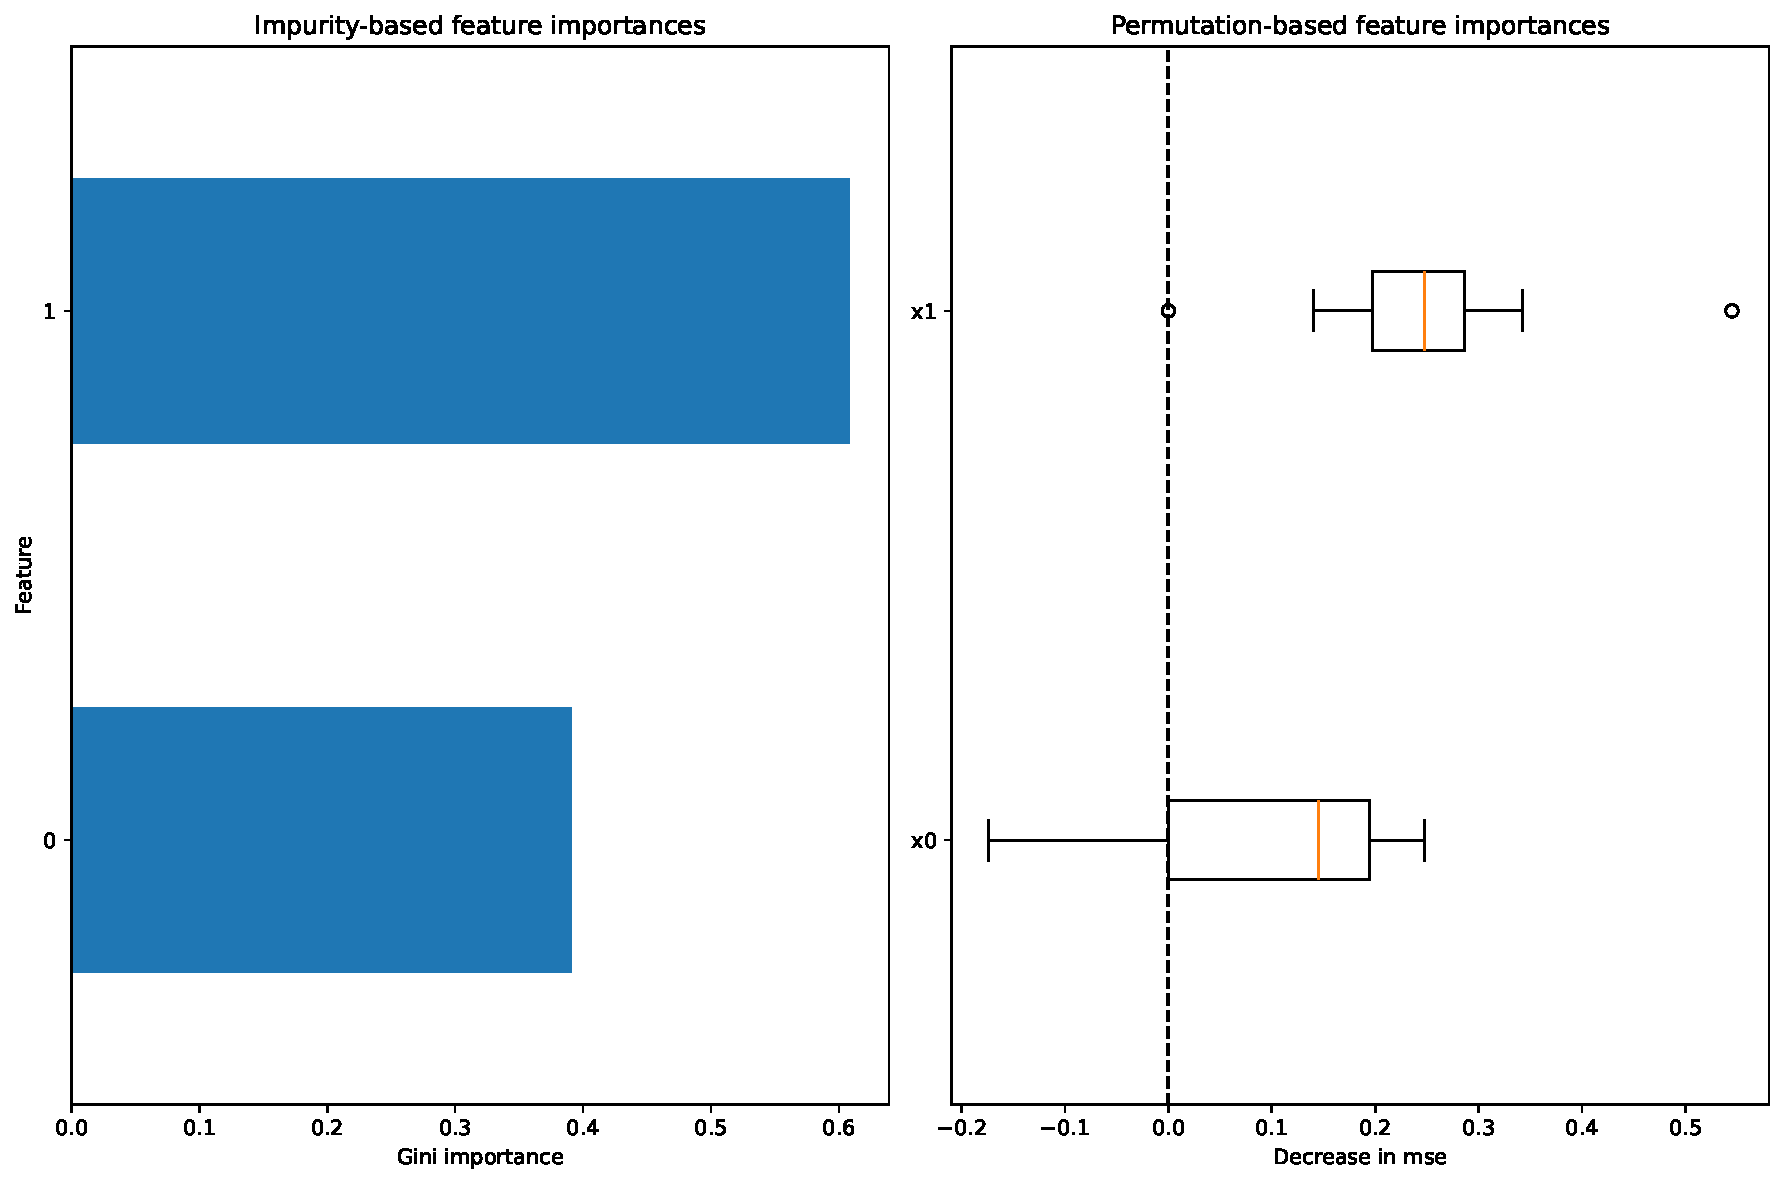
\includegraphics[keepaspectratio]{fig-importances-output-1.pdf}}

}

\caption{\label{fig-importances}Feature importances for the sphere
optimization. Left: impurity-based (Gini) importances from a Random
Forest. Right: permutation importances on the test set.}

\end{figure}%

Figure~\ref{fig-actual-vs-predicted} compares the surrogate's
predictions against the true objective values for all evaluated points.
The left panel shows actual versus predicted values (points on the
diagonal indicate perfect agreement); the right panel shows residuals
versus predicted values.

\begin{Shaded}
\begin{Highlighting}[]
\ImportTok{from}\NormalTok{ spotoptim.inspection }\ImportTok{import}\NormalTok{ (}
\NormalTok{    plot\_actual\_vs\_predicted}
\NormalTok{)}

\NormalTok{y\_pred }\OperatorTok{=}\NormalTok{ opt.surrogate.predict(opt.X\_)}
\NormalTok{plot\_actual\_vs\_predicted(opt.y\_, y\_pred, show}\OperatorTok{=}\VariableTok{False}\NormalTok{)}
\end{Highlighting}
\end{Shaded}

\begin{figure}[H]

\centering{

\pandocbounded{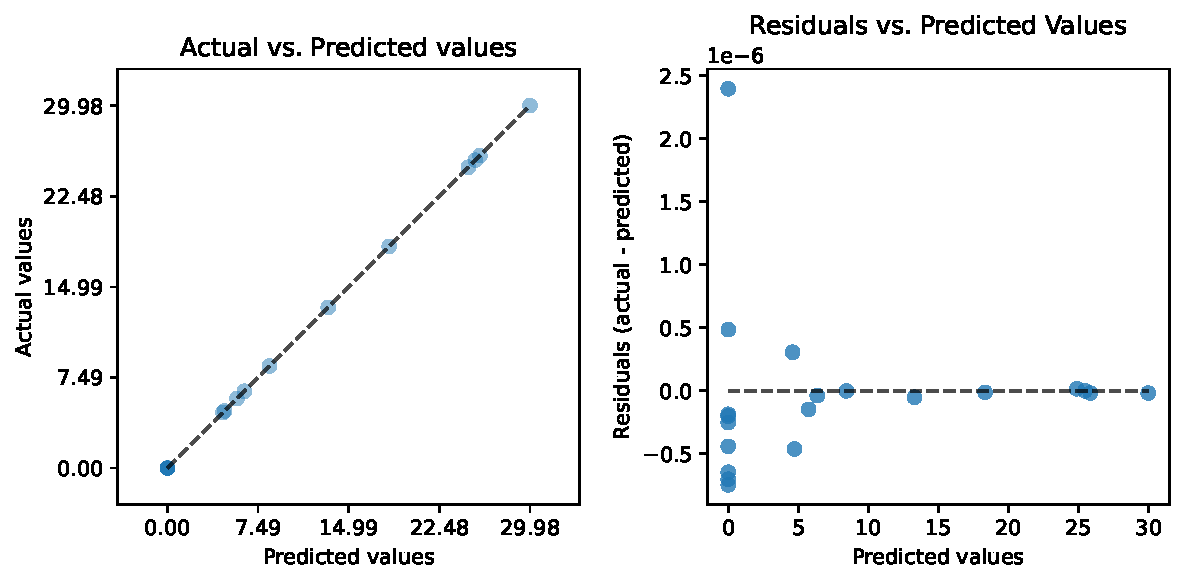
\includegraphics[keepaspectratio]{fig-actual-vs-predicted-output-1.pdf}}

}

\caption{\label{fig-actual-vs-predicted}Surrogate prediction
diagnostics. Left: actual versus predicted objective values. Right:
residuals versus predicted values.}

\end{figure}%

\subsection{Factor Analysis}\label{sec-factor}

The \texttt{factor\_analyzer} subpackage provides tools for exploratory
factor analysis of high-dimensional optimization data. It is a port of
the \texttt{factor\_analyzer} package for Python\footnote{\url{https://factor-analyzer.readthedocs.io/en/latest/index.html}}.
Before running the analysis, suitability tests (\texttt{calculate\_kmo}
for the Kaiser-Meyer-Olkin measure,
\texttt{calculate\_bartlett\_sphericity} for Bartlett's test) check
whether the data has sufficient correlational structure. The
\texttt{FactorAnalyzer} class extracts latent factors with optional
varimax or promax rotation, helping to reveal the latent structure in
large parameter spaces.

\subsection{Exploratory Data Analysis}\label{sec-eda}

The \texttt{eda} subpackage provides quick visualization functions for
inspecting optimization data. \texttt{plot\_ip\_histograms()} creates a
grid of histograms for each variable, with categorical variables shown
as bar charts. Specific configurations (such as the best solution) can
be overlaid as vertical lines using the \texttt{add\_points} parameter.

\subsection{Triangulation Candidates}\label{sec-tricands}

The \texttt{tricands} module generates candidate points for acquisition
optimization by computing the Delaunay triangulation of existing
evaluated points (Gramacy et al. 2022). Interior candidates are placed
at simplex centroids, exploring gaps between existing evaluations.
Fringe candidates extend beyond the convex hull toward the search space
boundary, encouraging exploration of unexplored regions. The \texttt{p}
parameter controls the extension fraction, and \texttt{nmax} limits the
total number of candidates. This geometry-aware approach complements the
global search performed by differential evolution and is particularly
effective in low-to-moderate dimensions where the triangulation remains
computationally tractable.

\section{Hyperparameter Tuning with spotoptim}\label{sec-hpt}

A primary application of \texttt{spotoptim} is the tuning of machine
learning hyperparameters, where each function evaluation corresponds to
training and validating a model with a specific configuration. This
section demonstrates a complete neural network tuning workflow using the
diabetes regression dataset, a multi-layer perceptron architecture, and
the \texttt{spotoptim} optimization loop. To keep execution time
manageable, the number of training epochs and optimization iterations
has been reduced. In practice, longer training runs (50--200 epochs per
evaluation) and larger evaluation budgets (\texttt{max\_iter}
\(\geq 30\)) are necessary to obtain reliable results. The short
configuration used here is intended solely as a demonstration of the
workflow and API; the best hyperparameters found in such a short run
should not be considered representative.

The workflow follows five steps: define the search space, prepare the
dataset, define the objective function, run the optimization, and
analyze the results. This structure mirrors the hyperparameter tuning
methodology described in Bartz et al. (2022) and Bartz-Beielstein and
Zaefferer (2022), now implemented entirely in Python.

\subsection{Defining the Search Space}\label{defining-the-search-space}

The search space is defined using a \texttt{ParameterSet} that specifies
the hyperparameters to tune, their types, bounds, and transformations:

\begin{Shaded}
\begin{Highlighting}[]
\ImportTok{from}\NormalTok{ spotoptim.hyperparameters }\OperatorTok{\textbackslash{}}
\NormalTok{    .parameters }\ImportTok{import}\NormalTok{ ParameterSet}

\NormalTok{ps\_hpt }\OperatorTok{=}\NormalTok{ ParameterSet()}
\NormalTok{ps\_hpt.add\_float(}\StringTok{"lr"}\NormalTok{, low}\OperatorTok{=}\FloatTok{1e{-}5}\NormalTok{, high}\OperatorTok{=}\FloatTok{0.1}\NormalTok{,}
\NormalTok{    default}\OperatorTok{=}\FloatTok{0.001}\NormalTok{, transform}\OperatorTok{=}\StringTok{"log10"}\NormalTok{)}
\NormalTok{ps\_hpt.add\_int(}\StringTok{"l1"}\NormalTok{, low}\OperatorTok{=}\DecValTok{8}\NormalTok{, high}\OperatorTok{=}\DecValTok{128}\NormalTok{,}
\NormalTok{    default}\OperatorTok{=}\DecValTok{32}\NormalTok{)}
\NormalTok{ps\_hpt.add\_int(}\StringTok{"num\_hidden\_layers"}\NormalTok{,}
\NormalTok{    low}\OperatorTok{=}\DecValTok{1}\NormalTok{, high}\OperatorTok{=}\DecValTok{4}\NormalTok{, default}\OperatorTok{=}\DecValTok{2}\NormalTok{)}
\NormalTok{ps\_hpt.add\_float(}\StringTok{"dropout"}\NormalTok{, low}\OperatorTok{=}\FloatTok{0.0}\NormalTok{,}
\NormalTok{    high}\OperatorTok{=}\FloatTok{0.5}\NormalTok{, default}\OperatorTok{=}\FloatTok{0.1}\NormalTok{)}
\ControlFlowTok{for}\NormalTok{ n, t, b }\KeywordTok{in} \BuiltInTok{zip}\NormalTok{(}
\NormalTok{    ps\_hpt.names(),}
\NormalTok{    ps\_hpt.var\_type,}
\NormalTok{    ps\_hpt.bounds,}
\NormalTok{):}
    \BuiltInTok{print}\NormalTok{(}\SpecialStringTok{f"}\SpecialCharTok{\{}\NormalTok{n}\SpecialCharTok{\}}\SpecialStringTok{ (}\SpecialCharTok{\{}\NormalTok{t}\SpecialCharTok{\}}\SpecialStringTok{): }\SpecialCharTok{\{}\NormalTok{b}\SpecialCharTok{\}}\SpecialStringTok{"}\NormalTok{)}
\end{Highlighting}
\end{Shaded}

\begin{verbatim}
lr (float): (1e-05, 0.1)
l1 (int): (8, 128)
num_hidden_layers (int): (1, 4)
dropout (float): (0.0, 0.5)
\end{verbatim}

The learning rate bounds are specified in natural scale
(\([10^{-5}, 10^{-1}]\)); the \texttt{log10} transformation tells
SpotOptim to work internally in log space, so the surrogate models a
smooth landscape. SpotOptim automatically converts back to natural scale
before calling the objective function. The \texttt{ParameterSet}
properties (\texttt{ps\_hpt.bounds}, \texttt{ps\_hpt.var\_type},
\texttt{ps\_hpt.names()}, \texttt{ps\_hpt.var\_trans}) map directly to
the \texttt{SpotOptim} constructor arguments.

\subsection{Preparing the Dataset}\label{preparing-the-dataset}

The diabetes dataset is loaded and split into training and test sets
using the provided data loader utility:

\begin{Shaded}
\begin{Highlighting}[]
\ImportTok{from}\NormalTok{ spotoptim.data }\ImportTok{import}\NormalTok{ (}
\NormalTok{    get\_diabetes\_dataloaders,}
\NormalTok{)}

\NormalTok{train\_loader, test\_loader, scaler }\OperatorTok{=}\NormalTok{ (}
\NormalTok{    get\_diabetes\_dataloaders(}
\NormalTok{        test\_size}\OperatorTok{=}\FloatTok{0.2}\NormalTok{,}
\NormalTok{        batch\_size}\OperatorTok{=}\DecValTok{32}\NormalTok{,}
\NormalTok{        scale\_features}\OperatorTok{=}\VariableTok{True}\NormalTok{,}
\NormalTok{        random\_state}\OperatorTok{=}\DecValTok{0}\NormalTok{,}
\NormalTok{    )}
\NormalTok{)}
\BuiltInTok{print}\NormalTok{(}\SpecialStringTok{f"Training batches: }\SpecialCharTok{\{}\BuiltInTok{len}\NormalTok{(train\_loader)}\SpecialCharTok{\}}\SpecialStringTok{"}\NormalTok{)}
\BuiltInTok{print}\NormalTok{(}\SpecialStringTok{f"Test batches: }\SpecialCharTok{\{}\BuiltInTok{len}\NormalTok{(test\_loader)}\SpecialCharTok{\}}\SpecialStringTok{"}\NormalTok{)}
\end{Highlighting}
\end{Shaded}

\begin{verbatim}
Training batches: 12
Test batches: 3
\end{verbatim}

The \texttt{scale\_features=True} option standardizes input features to
zero mean and unit variance, which is important for neural network
training stability.

\subsection{Defining the Objective
Function}\label{defining-the-objective-function}

The objective function decodes hyperparameters from the search vector,
constructs a \texttt{LinearRegressor}, trains it on the training set,
and returns the mean squared error (MSE) on the test set. Because
SpotOptim applies the inverse of \texttt{var\_trans} before calling the
objective, the learning rate arrives in natural scale and can be used
directly. The number of epochs is set to 10 for this demo; production
runs should use 50--200.

\begin{Shaded}
\begin{Highlighting}[]
\ImportTok{import}\NormalTok{ numpy }\ImportTok{as}\NormalTok{ np}
\ImportTok{import}\NormalTok{ torch}
\ImportTok{from}\NormalTok{ spotoptim.nn }\ImportTok{import}\NormalTok{ LinearRegressor}

\NormalTok{N\_EPOCHS }\OperatorTok{=} \DecValTok{10}  \CommentTok{\# short demo; use 50{-}200}

\KeywordTok{def}\NormalTok{ nn\_objective(X):}
\NormalTok{    X }\OperatorTok{=}\NormalTok{ np.atleast\_2d(X)}
\NormalTok{    results }\OperatorTok{=}\NormalTok{ np.zeros(X.shape[}\DecValTok{0}\NormalTok{])}
    \ControlFlowTok{for}\NormalTok{ i }\KeywordTok{in} \BuiltInTok{range}\NormalTok{(X.shape[}\DecValTok{0}\NormalTok{]):}
\NormalTok{        lr }\OperatorTok{=}\NormalTok{ X[i, }\DecValTok{0}\NormalTok{]}
\NormalTok{        l1 }\OperatorTok{=} \BuiltInTok{int}\NormalTok{(X[i, }\DecValTok{1}\NormalTok{])}
\NormalTok{        n\_layers }\OperatorTok{=} \BuiltInTok{int}\NormalTok{(X[i, }\DecValTok{2}\NormalTok{])}
\NormalTok{        dropout }\OperatorTok{=}\NormalTok{ X[i, }\DecValTok{3}\NormalTok{]}
\NormalTok{        model }\OperatorTok{=}\NormalTok{ LinearRegressor(}
\NormalTok{            input\_dim}\OperatorTok{=}\DecValTok{10}\NormalTok{, output\_dim}\OperatorTok{=}\DecValTok{1}\NormalTok{,}
\NormalTok{            l1}\OperatorTok{=}\NormalTok{l1,}
\NormalTok{            num\_hidden\_layers}\OperatorTok{=}\NormalTok{n\_layers,}
\NormalTok{            activation}\OperatorTok{=}\StringTok{"ReLU"}\NormalTok{,}
\NormalTok{        )}
\NormalTok{        opt }\OperatorTok{=}\NormalTok{ torch.optim.Adam(}
\NormalTok{            model.parameters(), lr}\OperatorTok{=}\NormalTok{lr)}
\NormalTok{        loss\_fn }\OperatorTok{=}\NormalTok{ torch.nn.MSELoss()}
\NormalTok{        model.train()}
        \ControlFlowTok{for}\NormalTok{ epoch }\KeywordTok{in} \BuiltInTok{range}\NormalTok{(N\_EPOCHS):}
            \ControlFlowTok{for}\NormalTok{ xb, yb }\KeywordTok{in}\NormalTok{ train\_loader:}
\NormalTok{                opt.zero\_grad()}
\NormalTok{                loss }\OperatorTok{=}\NormalTok{ loss\_fn(model(xb), yb)}
\NormalTok{                loss.backward()}
\NormalTok{                opt.step()}
\NormalTok{        model.}\BuiltInTok{eval}\NormalTok{()}
\NormalTok{        total\_loss, n }\OperatorTok{=} \FloatTok{0.0}\NormalTok{, }\DecValTok{0}
        \ControlFlowTok{with}\NormalTok{ torch.no\_grad():}
            \ControlFlowTok{for}\NormalTok{ xb, yb }\KeywordTok{in}\NormalTok{ test\_loader:}
\NormalTok{                total\_loss }\OperatorTok{+=}\NormalTok{ (}
\NormalTok{                    loss\_fn(model(xb), yb)}
\NormalTok{                    .item() }\OperatorTok{*} \BuiltInTok{len}\NormalTok{(yb))}
\NormalTok{                n }\OperatorTok{+=} \BuiltInTok{len}\NormalTok{(yb)}
\NormalTok{        results[i] }\OperatorTok{=}\NormalTok{ total\_loss }\OperatorTok{/}\NormalTok{ n}
    \ControlFlowTok{return}\NormalTok{ results}
\end{Highlighting}
\end{Shaded}

The function follows \texttt{spotoptim}'s convention: it accepts a 2-D
array where each row is a configuration and returns a 1-D array of
objective values.

\subsection{Running the Optimization}\label{running-the-optimization}

With the search space and objective function defined, the optimization
is launched with a single call. The optimizer is configured with
Expected Improvement and a small budget suitable for a demo. Production
runs should increase \texttt{max\_iter} to 30 or more.

\begin{Shaded}
\begin{Highlighting}[]
\ImportTok{from}\NormalTok{ spotoptim }\ImportTok{import}\NormalTok{ SpotOptim}

\NormalTok{opt\_hpt }\OperatorTok{=}\NormalTok{ SpotOptim(}
\NormalTok{    fun}\OperatorTok{=}\NormalTok{nn\_objective,}
\NormalTok{    bounds}\OperatorTok{=}\NormalTok{ps\_hpt.bounds,}
\NormalTok{    var\_type}\OperatorTok{=}\NormalTok{ps\_hpt.var\_type,}
\NormalTok{    var\_name}\OperatorTok{=}\NormalTok{ps\_hpt.names(),}
\NormalTok{    var\_trans}\OperatorTok{=}\NormalTok{ps\_hpt.var\_trans,}
\NormalTok{    acquisition}\OperatorTok{=}\StringTok{"ei"}\NormalTok{,}
\NormalTok{    max\_iter}\OperatorTok{=}\DecValTok{15}\NormalTok{, n\_initial}\OperatorTok{=}\DecValTok{8}\NormalTok{, seed}\OperatorTok{=}\DecValTok{0}\NormalTok{,}
\NormalTok{)}
\NormalTok{result\_hpt }\OperatorTok{=}\NormalTok{ opt\_hpt.optimize()}

\BuiltInTok{print}\NormalTok{(}\SpecialStringTok{f"Best MSE: }\SpecialCharTok{\{}\NormalTok{result\_hpt}\SpecialCharTok{.}\NormalTok{fun}\SpecialCharTok{:.4f\}}\SpecialStringTok{"}\NormalTok{)}
\BuiltInTok{print}\NormalTok{(}\SpecialStringTok{f"Evaluations: }\SpecialCharTok{\{}\NormalTok{result\_hpt}\SpecialCharTok{.}\NormalTok{nfev}\SpecialCharTok{\}}\SpecialStringTok{"}\NormalTok{)}
\BuiltInTok{print}\NormalTok{(}\StringTok{"Best config:"}\NormalTok{)}
\ControlFlowTok{for}\NormalTok{ n, v }\KeywordTok{in} \BuiltInTok{zip}\NormalTok{(}
\NormalTok{    ps\_hpt.names(), result\_hpt.x}
\NormalTok{):}
    \BuiltInTok{print}\NormalTok{(}\SpecialStringTok{f"  }\SpecialCharTok{\{}\NormalTok{n}\SpecialCharTok{\}}\SpecialStringTok{: }\SpecialCharTok{\{}\NormalTok{v}\SpecialCharTok{:.6g\}}\SpecialStringTok{"}\NormalTok{)}
\end{Highlighting}
\end{Shaded}

\begin{verbatim}
Best MSE: 3534.6855
Evaluations: 15
Best config:
  lr: 0.025114
  l1: 88
  num_hidden_layers: 2
  dropout: 0.408088
\end{verbatim}

The Kriging surrogate builds a model of the validation loss as a
function of the hyperparameters, and Expected Improvement guides the
search toward configurations that are either predicted to perform well
or that have high uncertainty.

\subsection{Analyzing the Results}\label{analyzing-the-results}

After optimization, the reporting utilities summarize which
hyperparameters were most influential and display the best
configuration. The progress plot (Figure~\ref{fig-hpt-progress}) shows
the convergence of the optimization.

\begin{Shaded}
\begin{Highlighting}[]
\ImportTok{from}\NormalTok{ spotoptim.plot.visualization }\ImportTok{import}\NormalTok{ (}
\NormalTok{    plot\_progress,}
\NormalTok{)}
\NormalTok{plot\_progress(opt\_hpt, show}\OperatorTok{=}\VariableTok{False}\NormalTok{, log\_y}\OperatorTok{=}\VariableTok{True}\NormalTok{)}
\end{Highlighting}
\end{Shaded}

\begin{figure}[H]

\centering{

\pandocbounded{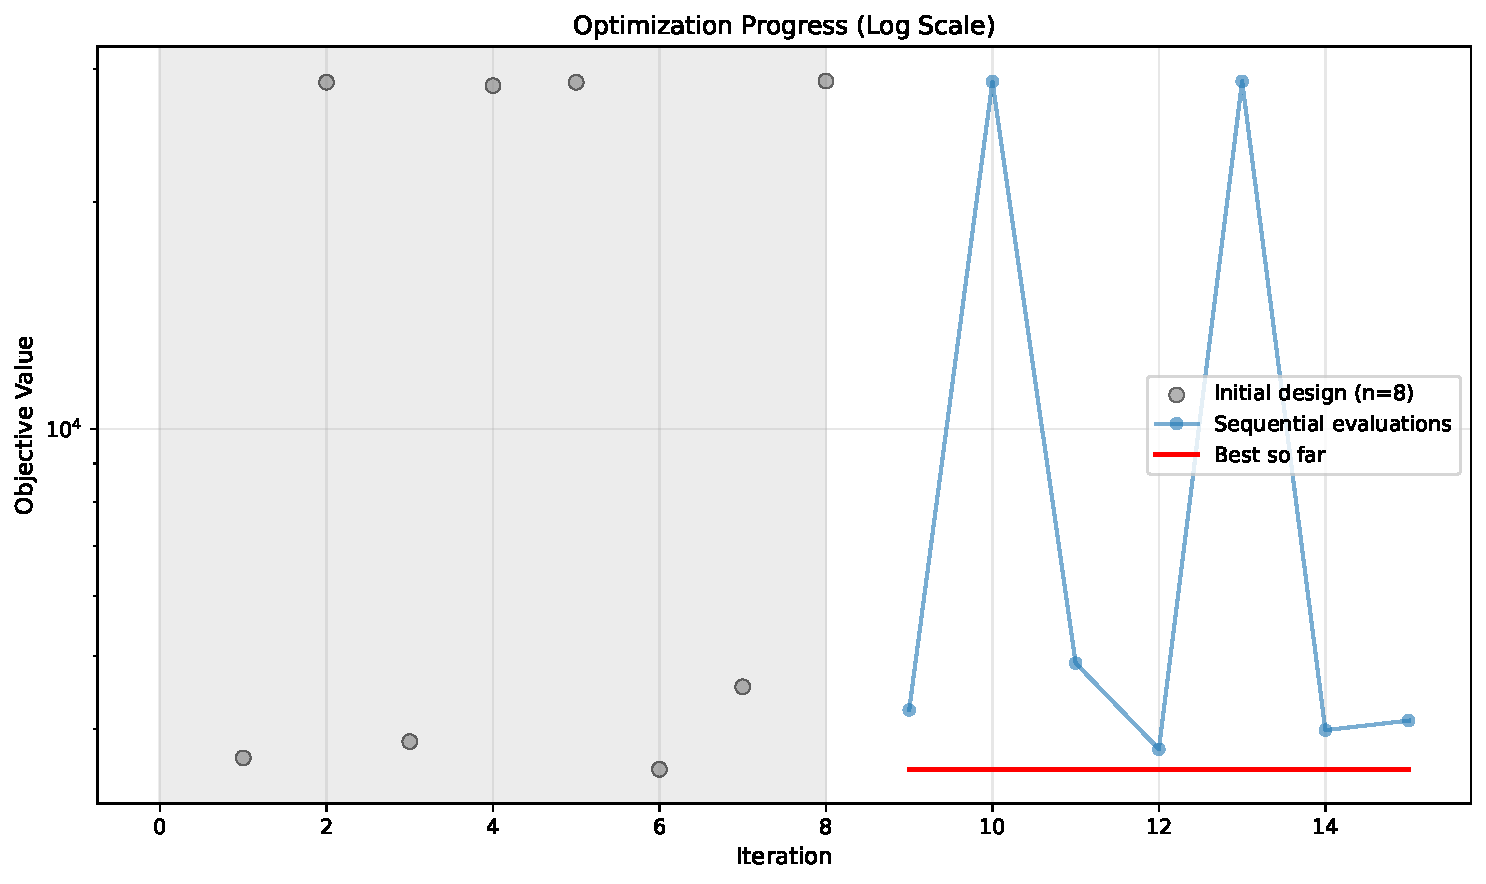
\includegraphics[keepaspectratio]{fig-hpt-progress-output-1.pdf}}

}

\caption{\label{fig-hpt-progress}Hyperparameter tuning progress (demo
run with reduced epochs and budget). The red curve shows the best
validation MSE found so far.}

\end{figure}%

The feature importances (Figure~\ref{fig-hpt-importances}) reveal which
hyperparameters had the strongest influence on the validation loss.

\begin{Shaded}
\begin{Highlighting}[]
\ImportTok{from}\NormalTok{ sklearn.model\_selection }\ImportTok{import}\NormalTok{ (}
\NormalTok{    train\_test\_split,}
\NormalTok{)}
\ImportTok{from}\NormalTok{ spotoptim.inspection }\ImportTok{import}\NormalTok{ (}
\NormalTok{    generate\_mdi, generate\_imp,}
\NormalTok{    plot\_importances,}
\NormalTok{)}

\NormalTok{X\_tr, X\_te, y\_tr, y\_te }\OperatorTok{=}\NormalTok{ train\_test\_split(}
\NormalTok{    opt\_hpt.X\_, opt\_hpt.y\_,}
\NormalTok{    test\_size}\OperatorTok{=}\FloatTok{0.3}\NormalTok{, random\_state}\OperatorTok{=}\DecValTok{42}\NormalTok{,}
\NormalTok{)}
\NormalTok{df\_mdi }\OperatorTok{=}\NormalTok{ generate\_mdi(}
\NormalTok{    X\_tr, y\_tr,}
\NormalTok{    feature\_names}\OperatorTok{=}\NormalTok{ps\_hpt.names(),}
\NormalTok{)}
\NormalTok{perm\_imp }\OperatorTok{=}\NormalTok{ generate\_imp(}
\NormalTok{    X\_tr, X\_te, y\_tr, y\_te,}
\NormalTok{)}
\NormalTok{plot\_importances(}
\NormalTok{    df\_mdi, perm\_imp, X\_te,}
\NormalTok{    feature\_names}\OperatorTok{=}\NormalTok{ps\_hpt.names(),}
\NormalTok{    show}\OperatorTok{=}\VariableTok{False}\NormalTok{,}
\NormalTok{)}
\end{Highlighting}
\end{Shaded}

\begin{figure}[H]

\centering{

\pandocbounded{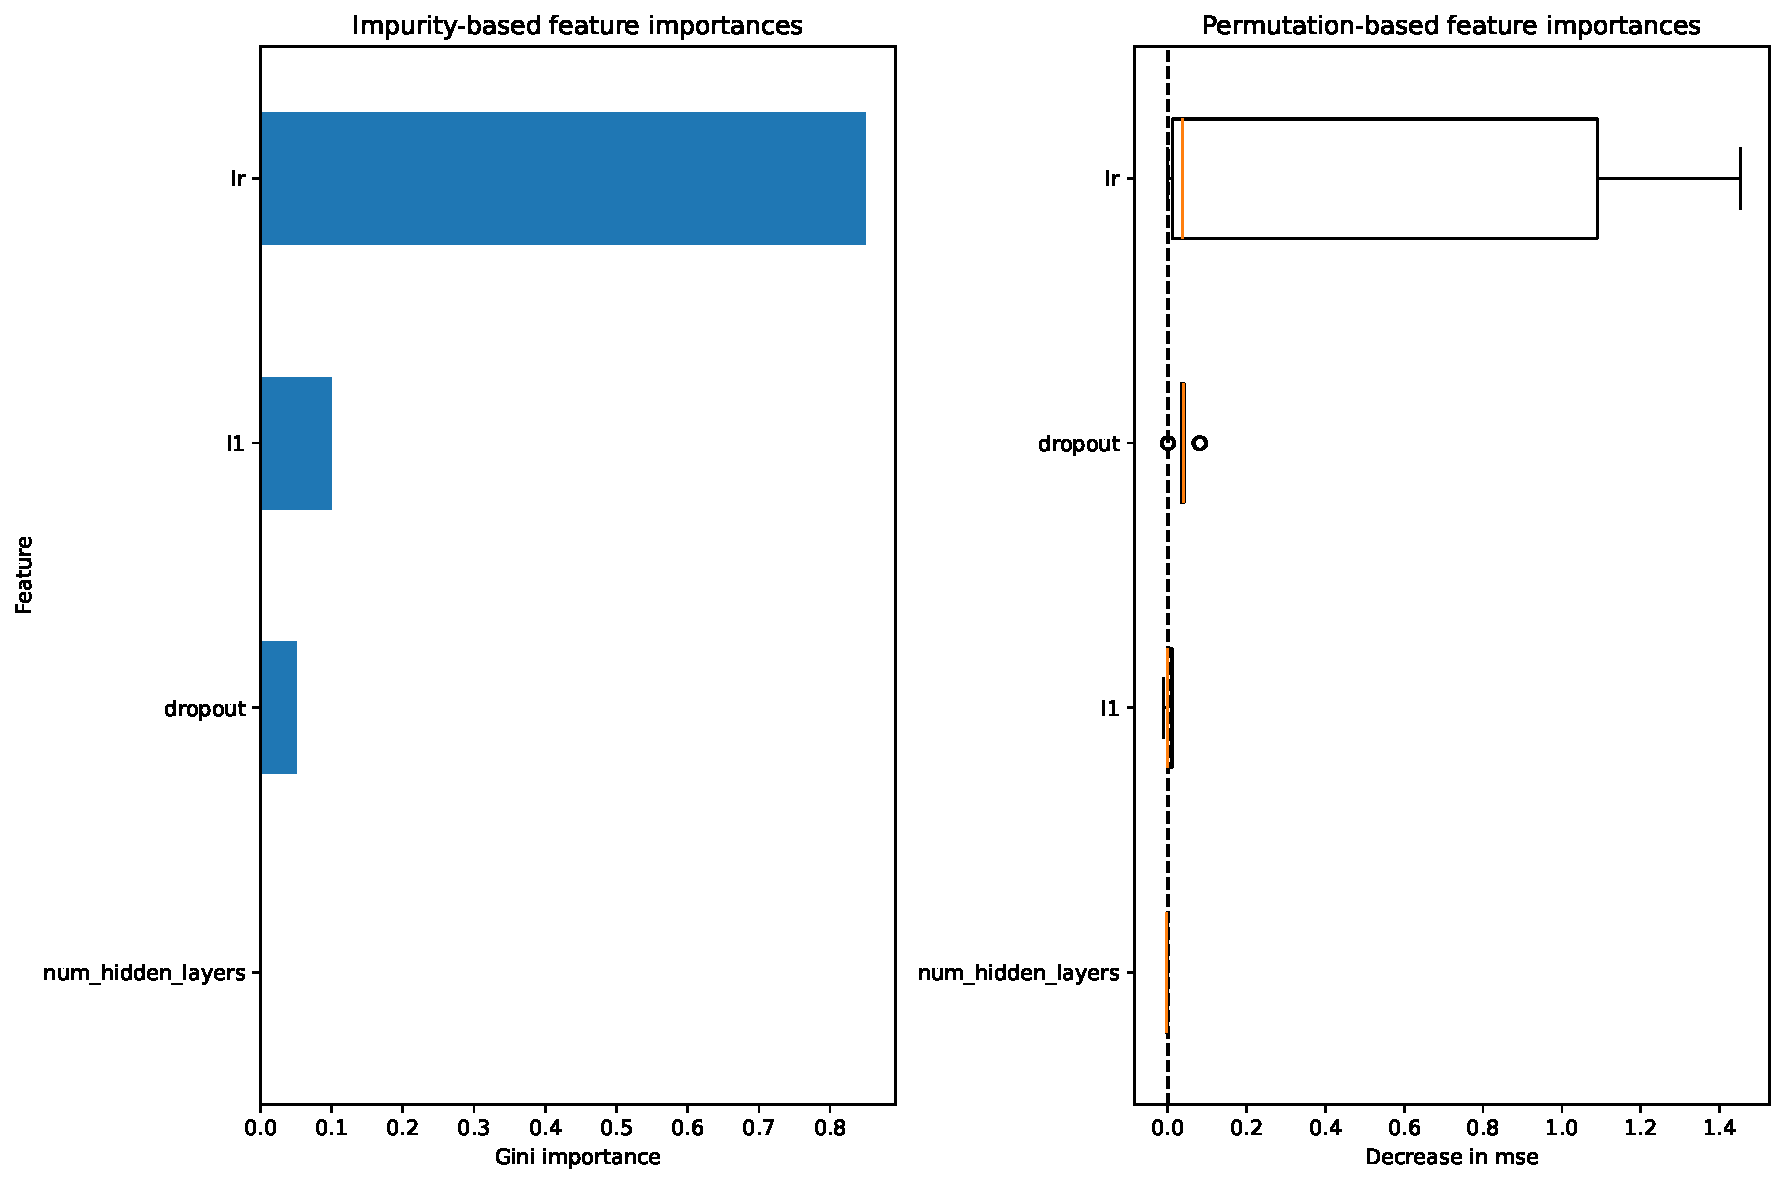
\includegraphics[keepaspectratio]{fig-hpt-importances-output-1.pdf}}

}

\caption{\label{fig-hpt-importances}Feature importances for the
hyperparameter tuning demo. Left: impurity-based (Gini) importances.
Right: permutation importances on the test set.}

\end{figure}%

The \texttt{sensitivity\_spearman} function reports Spearman rank
correlations between each hyperparameter and the objective value, with
significance stars indicating statistical confidence. This helps the
practitioner understand which hyperparameters merit further
investigation and which can be fixed at their default values.

\begin{Shaded}
\begin{Highlighting}[]
\ImportTok{from}\NormalTok{ spotoptim.reporting.analysis }\ImportTok{import}\NormalTok{ (}
\NormalTok{    sensitivity\_spearman,}
\NormalTok{)}
\NormalTok{sensitivity\_spearman(opt\_hpt)}
\end{Highlighting}
\end{Shaded}

\begin{verbatim}

Sensitivity Analysis (Spearman Correlation):
--------------------------------------------------
  lr                  : -0.676 (p=0.006) **
  l1                  : -0.454 (p=0.089)
  num_hidden_layers   : +0.074 (p=0.794)
  dropout             : -0.533 (p=0.041) *
\end{verbatim}

The complete workflow described here can be compared with the
corresponding Ray Tune setup documented by Bartz-Beielstein (2023b).
While Ray Tune provides distributed scheduling across multiple machines,
\texttt{spotoptim} offers a more transparent, model-centric approach
where the user controls the surrogate model, acquisition function, and
experimental design. For single-machine workflows with moderate
evaluation budgets (tens to hundreds of configurations), the
surrogate-based approach is typically more sample-efficient than the
random or bandit-based strategies employed by Ray Tune's default
schedulers.

\section{Summary and Outlook}\label{sec-outlook}

This paper has presented \texttt{spotoptim}, a Python package for
surrogate-model-based optimization of expensive black-box functions. The
package implements the Sequential Parameter Optimization methodology
with Kriging as the default surrogate, Expected Improvement and related
acquisition functions, native support for mixed variable types,
noise-aware evaluation through repeated evaluations and OCBA, and
multi-objective extensions via Pareto analysis and desirability
functions. The architecture is designed around scikit-learn
compatibility for surrogates and scipy compatibility for results, making
the package interoperable with the broader Python scientific computing
ecosystem.

\texttt{spotoptim} represents the current generation of a two-decade
research lineage. It uses a modular architecture, structural typing
protocols, and comprehensive documentation. The package is part of an
ecosystem of related tools. For example, \texttt{spotdesirability}
provides desirability functions for multi-objective optimization,
enabling the user to express preferences over multiple objectives
through individual desirability curves and overall aggregation
(Bartz-Beielstein 2025a, 2025b), \texttt{spotforecast2} extends the
optimization framework to time-series forecasting, and
\texttt{spotforecast2\_safe} adds robustness guarantees for
safety-critical forecasting applications. The emergence of free-threaded
Python opens the possibility of true thread-level parallelism for
objective evaluation; \texttt{spotoptim} already includes a
\texttt{is\_gil\_disabled()} check that detects free-threaded builds and
can adapt its parallelism strategy accordingly. The \texttt{spotoptim}
package is open-source and available at
\url{https://github.com/sequential-parameter-optimization/spotoptim}
under the AGPL-3.0 license. Documentation, including an API reference
and a comprehensive user guide with executable code examples, is hosted
at \url{https://sequential-parameter-optimization.github.io/spotoptim/}.

\section*{References}\label{references}
\addcontentsline{toc}{section}{References}

\protect\phantomsection\label{refs}
\begin{CSLReferences}{1}{1}
\bibitem[\citeproctext]{ref-akib19a}
Akiba, Takuya, Shotaro Sano, Toshihiko Yanase, Takeru Ohta, and Masanori
Koyama. 2019. {``{Optuna: A Next-generation Hyperparameter Optimization
Framework}.''} \emph{Proceedings of the 25th ACM SIGKDD International
Conference on Knowledge Discovery \& Data Mining}, 2623--31.
\url{https://doi.org/10.1145/3292500.3330701}.

\bibitem[\citeproctext]{ref-bala20a}
Balandat, Maximilian, Brian Karrer, Daniel R. Jiang, et al. 2020.
{``{BoTorch: A Framework for Efficient Monte-Carlo Bayesian
Optimization}.''} \emph{Advances in Neural Information Processing
Systems 33}. \url{https://arxiv.org/abs/1910.06403}.

\bibitem[\citeproctext]{ref-bart21i}
Bartz, Eva, Thomas Bartz-Beielstein, Martin Zaefferer, and Olaf
Mersmann, eds. 2022. \emph{{Hyperparameter Tuning for Machine and Deep
Learning with R - A Practical Guide}}. Springer.

\bibitem[\citeproctext]{ref-bart23iArXiv}
Bartz-Beielstein, Thomas. 2023a. {``{Hyperparameter Tuning Cookbook: A
guide for scikit-learn, PyTorch, river, and spotpython}.''} \emph{arXiv
e-Prints}, ahead of print, July.
\url{https://doi.org/10.48550/arXiv.2307.10262}.

\bibitem[\citeproctext]{ref-bart23e}
Bartz-Beielstein, Thomas. 2023b. \emph{{PyTorch} Hyperparameter Tuning
with {SPOT}: Comparison with {Ray Tuner} and Default Hyperparameters on
{CIFAR10}}.
\url{https://github.com/sequential-parameter-optimization/spotpython/blob/main/notebooks/14_spot_ray_hpt_torch_cifar10.ipynb}.

\bibitem[\citeproctext]{ref-bart25a}
Bartz-Beielstein, Thomas. 2025a. {``{Multi-Objective Optimization and
Hyperparameter Tuning With Desirability Functions}.''} \emph{arXiv
e-Prints}, March, arXiv:2503.23595.
\url{https://doi.org/10.48550/arXiv.2503.23595}.

\bibitem[\citeproctext]{ref-bart25b}
Bartz-Beielstein, Thomas. 2025b. {``Surrogate Model-Based
Multi-Objective Optimization Using Desirability Functions.''}
\emph{Proceedings of the Genetic and Evolutionary Computation Conference
Companion} (New York, NY, USA), GECCO '25 companion, 2458--65.
\url{https://doi.org/10.1145/3712255.3734331}.

\bibitem[\citeproctext]{ref-Bart11a}
Bartz-Beielstein, Thomas, and Martina Friese. 2011. \emph{{Sequential
Parameter Optimization and Optimal Computational Budget Allocation for
Noisy Optimization Problems}}. Cologne University of Applied Science,
Faculty of Computer Science; Engineering Science.

\bibitem[\citeproctext]{ref-Bart11b}
Bartz-Beielstein, Thomas, Martina Friese, Martin Zaefferer, et al. 2011.
{``{Noisy optimization with sequential parameter optimization and
optimal computational budget allocation}.''} \emph{Proceedings of the
13th Annual Conference Companion on Genetic and Evolutionary
Computation} (New York, NY, USA), 119--20.

\bibitem[\citeproctext]{ref-BLP05}
Bartz-Beielstein, Thomas, Christian Lasarczyk, and Mike Preuss. 2005.
{``{Sequential Parameter Optimization}.''} In \emph{{Proceedings 2005
Congress on Evolutionary Computation (CEC'05), Edinburgh, Scotland}},
{edited by B McKay et al.} {IEEE Press}.
\url{https://doi.org/10.1109/CEC.2005.1554761}.

\bibitem[\citeproctext]{ref-Bart16n}
Bartz-Beielstein, Thomas, and Martin Zaefferer. 2017. {``Model-Based
Methods for Continuous and Discrete Global Optimization.''}
\emph{Applied Soft Computing} 55: 154--67.
\url{https://doi.org/10.1016/j.asoc.2017.01.039}.

\bibitem[\citeproctext]{ref-bart21ic3}
Bartz-Beielstein, Thomas, and Martin Zaefferer. 2022. {``Hyperparameter
Tuning Approaches.''} Chap. 4 in \emph{{Hyperparameter Tuning for
Machine and Deep Learning with R - A Practical Guide}}, edited by Eva
Bartz, Thomas Bartz-Beielstein, Martin Zaefferer, and Olaf Mersmann.
Springer.

\bibitem[\citeproctext]{ref-bart21b}
Bartz-Beielstein, Thomas, Martin Zaefferer, and Frederik Rehbach. 2021.
{``{In a Nutshell -- The Sequential Parameter Optimization Toolbox}.''}
\emph{arXiv e-Prints}, December, arXiv:1712.04076.

\bibitem[\citeproctext]{ref-berg11a}
Bergstra, James, Rémi Bardenet, Yoshua Bengio, and Balázs Kégl. 2011.
{``{Algorithms for Hyper-Parameter Optimization}.''} \emph{Advances in
Neural Information Processing Systems} 24.

\bibitem[\citeproctext]{ref-Chen10a}
Chen, Chun Hung. 2010. \emph{{Stochastic simulation optimization: an
optimal computing budget allocation}}. World Scientific.

\bibitem[\citeproctext]{ref-falk18a}
Falkner, Stefan, Aaron Klein, and Frank Hutter. 2018. {``{BOHB: Robust
and Efficient Hyperparameter Optimization at Scale}.''}
\emph{Proceedings of the 35th International Conference on Machine
Learning}, 1437--46.

\bibitem[\citeproctext]{ref-Forr08a}
Forrester, Alexander, András Sóbester, and Andy Keane. 2008.
\emph{{Engineering Design via Surrogate Modelling}}. Wiley.

\bibitem[\citeproctext]{ref-Gent18a}
Gentile, Lorenzo, Thomas Bartz-Beielstein, and Martin Zaefferer. 2021.
{``Sequential Parameter Optimization for Mixed-Discrete Problems.''} In
\emph{Optimization Under Uncertainty with Applications to Aerospace
Engineering}, edited by Massimiliano Vasile. Springer International
Publishing. \url{https://doi.org/10.1007/978-3-030-60166-9_10}.

\bibitem[\citeproctext]{ref-Gent18b}
Gentile, Lorenzo, Martin Zaefferer, Dario Giugliano, Haofeng Chen, and
Thomas Bartz-Beielstein. 2018. {``Surrogate Assisted Optimization of
Particle Reinforced Metal Matrix Composites.''} \emph{Proceedings of the
Genetic and Evolutionary Computation Conference} (New York, NY, USA),
GECCO '18, 1238--45. \url{https://doi.org/10.1145/3205455.3205574}.

\bibitem[\citeproctext]{ref-Gram20a}
Gramacy, Robert B. 2020. \emph{Surrogates}. {CRC} press.

\bibitem[\citeproctext]{ref-gram22a}
Gramacy, Robert B., Annie Sauer, and Nathan Wycoff. 2022.
\emph{Triangulation Candidates for Bayesian Optimization}.
\url{https://arxiv.org/abs/2112.07457}.

\bibitem[\citeproctext]{ref-Hutt09a}
Hutter, Frank, Thomas Bartz-Beielstein, Holger Hoos, Kevin Leyton-Brown,
and Kevin P Murphy. 2010. {``{Sequential Model-Based Parameter
Optimisation: an Experimental Investigation of Automated and Interactive
Approaches}.''} In \emph{Experimental Methods for the Analysis of
Optimization Algorithms}, edited by Thomas Bartz-Beielstein, Marco
Chiarandini, Luis Paquete, and Mike Preuss. Springer.

\bibitem[\citeproctext]{ref-hutt11a}
Hutter, Frank, Holger H. Hoos, and Kevin Leyton-Brown. 2011.
{``{Sequential Model-based Algorithm Configuration}.''} \emph{Learning
and Intelligent Optimization (LION 5)}, 507--23.
\url{https://doi.org/10.1007/978-3-642-25566-3_40}.

\bibitem[\citeproctext]{ref-Jone98a}
Jones, D R, M Schonlau, and W J Welch. 1998. {``{Efficient Global
Optimization of Expensive Black-Box Functions}.''} \emph{Journal of
Global Optimization} 13: 455--92.

\bibitem[\citeproctext]{ref-jones98a}
Jones, Donald R., Matthias Schonlau, and William J. Welch. 1998.
{``{Efficient Global Optimization of Expensive Black-Box Functions}.''}
\emph{Journal of Global Optimization} 13 (4): 455--92.
\url{https://doi.org/10.1023/A:1008306431147}.

\bibitem[\citeproctext]{ref-liaw18a}
Liaw, Richard, Eric Liang, Robert Nishihara, Philipp Moritz, Roy Fox,
and Ken Goldberg. 2018. {``{Tune: A Research Platform for Distributed
Model Selection and Training}.''} \emph{ICML AutoML Workshop}.
\url{https://arxiv.org/abs/1807.05118}.

\bibitem[\citeproctext]{ref-Stor96a}
Storn, R. 1996. {``{On the usage of differential evolution for function
optimization}.''} \emph{Fuzzy Information Processing Society, 1996.
NAFIPS., 1996 Biennial Conference of the North American}, 519--23.
\url{https://doi.org/10.1109/NAFIPS.1996.534789}.

\bibitem[\citeproctext]{ref-Zaef16b}
Zaefferer, Martin, and Thomas Bartz-Beielstein. 2016. {``Efficient
Global Optimization with Indefinite Kernels.''} In \emph{Parallel
Problem Solving from Nature -- PPSN XIV: 14th International Conference,
Edinburgh, UK, September 17-21, 2016, Proceedings}, edited by Julia
Handl, Emma Hart, Peter R. Lewis, Manuel López-Ibáñez, Gabriela Ochoa,
and Ben Paechter. Springer International Publishing.
\url{https://doi.org/10.1007/978-3-319-45823-6_7}.

\bibitem[\citeproctext]{ref-Zaef14c}
Zaefferer, Martin, Jörg Stork, and Thomas Bartz-Beielstein. 2014.
{``{Distance Measures for Permutations in Combinatorial Efficient Global
Optimization}.''} In \emph{Parallel Problem Solving from Nature--PPSN
XIII}, edited by Thomas Bartz-Beielstein, Jürgen Branke, Bogdan Filipic,
and Jim Smith. Springer.

\bibitem[\citeproctext]{ref-Zaef14b}
Zaefferer, Martin, Jörg Stork, Martina Friese, Andreas Fischbach, Boris
Naujoks, and Thomas Bartz-Beielstein. 2014. {``{Efficient Global
Optimization for Combinatorial Problems}.''} In \emph{Genetic and
Evolutionary Computation Conference (GECCO'14), Proceedings}, edited by
Dirk V Arnold. ACM.
https://doi.org/\url{http://doi.acm.org/10.1145/2576768.2598282}.

\end{CSLReferences}




\end{document}
